\section{Generation of haplotypes from raw reads}
Given the need to include large sample sizes from diverse populations for such a resource for development of an African chip, curation of data will involve generation of homogenised data from different datasets, including publicly available data as outlined in Table 1. Given the heterogeneity in sequencing and coverage among datasets (Table 1), these will need to be processed in subsets, and then merged to generate a complete panel of all variants. 

Publicly available curated data from the \href{http://www.1000genomes.org}{1000 Genomes project (1000G)}
%and the \href{http://www.simonsfoundation.org/}{Simon’s Foundation}
will be used as such. For datasets that are sequenced in house, consistent methods will be used for curation.

% Text written by Martin on 27jan2015
% Text modified by Tommy on 20apr2015

All sequence data generated in house will be processed homogeneously to avoid pipeline related artifacts.

\subsubsection{Alignment and preprocessing of reads}
Following generation of raw reads on the sequencing machine, the reads will be converted to BAM format using Illumina2BAM\footnote{https://github.com/wtsi-npg/illumina2bam}. Illumina2BAM will be used to de-multiplex the lanes that have been sequenced so that the tags are isolated from the body of the read, decoded, and can be used to separate out each lane into lanelets containing individual samples from the multiplex library and the PhiX control.  Reads corresponding to the PhiX control are mapped and used with Sanger’s spatial filter program\footnote{https://github.com/wtsi-npg/pb\_calibration} to identify reads from other lanelets that contain spatially oriented INDEL artefacts and mark them as QC fail. Mapping  of the Human samples is carried out using the BWA-MEM algorithm of the BWA software package, which is suitable for Illumina reads longer than 70bp\cite{2013arXiv1303.3997L}, with the GRCh37 1000 Genomes phase II reference (also known as hs37d5). PCR and optically duplicated reads are marked using Picard\footnote{http://broadinstitute.github.io/picard} MarkDuplicates.

\subsubsection{Quality control prior to variant calling}
In order to ensure the quality of the large quantity of BAMs produced for the project, an automatic quality control system is employed to reduce the number of data files that require manual intervention. This system has been derived from the one originally designed for the \href{http://www.uk10k.org}{UK10K  project} and uses a series of empirically derived thresholds to assess summary metrics calculated from the input BAMs. These thresholds include: percentage of reads mapped; percentage of duplicate reads marked; various statistics measuring indel distribution against read cycle and an insert size overlap percentage. Any lane that falls below the “fail” threshold for any of the metrics is excluded; any lane that falls below the “warn” threshold on a metric is manually examined; and any lane that does not fall below either of these thresholds for any of the metrics is given a status of “pass” and allowed to proceed into the later stages of the pipeline.
Table \ref{table:failQC} on page \pageref{table:failQC} summarises the samples failing the initial QC.
%http://hgi-www.internal.sanger.ac.uk/qc_grind/samples_view.pl?db=hgip_vrtrack_mercury_prod&proj_id=34
%http://hgi-www.internal.sanger.ac.uk/qc_grind/samples_view.pl?db=hgip_vrtrack_mercury_prod&proj_id=10
%http://hgi-www.internal.sanger.ac.uk/qc_grind/samples_view.pl?db=hgip_vrtrack_mercury_prod&proj_id=56
%http://hgi-www.internal.sanger.ac.uk/qc_grind/samples_view.pl?db=hgip_vrtrack_mercury_prod&proj_id=107
%http://hgi-www.internal.sanger.ac.uk/qc_grind/samples_view.pl?db=hgip_vrtrack_mercury_prod&proj_id=160
%http://hgi-www.internal.sanger.ac.uk/qc_grind/samples_view.pl?db=hgip_vrtrack_mercury_prod&proj_id=101
\begin{table}[htp]
\centering
\resizebox{\textwidth}{!}{%
\begin{tabular}{|l|l|l|l|l|l|l|}
\hline
Sequence ID & Chip ID & Sex & Ethnicity & seq QC & chip QC & Depth \\
\hline
EGAN00001069167 & APP5201664 & F & Zulu & Fail & Pass & N/A \\
EGAN00001069192 & APP5201736 & M & Zulu & Fail & Pass & N/A \\
EGAN00001160764 & APP5292683 & M & Baganda & Fail & Pass &  \\
EGAN00001160765 & APP5292684 & M & Baganda & Fail & Pass &  \\
EGAN00001160766 & APP5292685 & F & Baganda & Fail & Pass &  \\
EGAN00001161026 & APP5292945 & F & Baganda & Fail & Pass &  \\
EGAN00001161719 & APP5293638 & M & RwandeseUgandan & Fail & Pass &  \\
EGAN00001163789 & APP5340012 & M & Baganda & Fail & Pass &  \\
EGAN00001164177 & APP5340400 & F & Banyarwanda & Fail & Pass &  \\
EGAN00001164349 & APP5340572 & F & Baganda & Fail & Pass &  \\
EGAN00001164578 & APP5340801 & F & Baganda & Fail & Pass &  \\
EGAN00001164611 & APP5340834 & M & Baganda & Fail & Pass &  \\
EGAN00001164939 & APP5341162 & F & Baganda & Fail & Pass &  \\
EGAN00001164957 & APP5341180 & M & Baganda & Fail & Pass &  \\
EGAN00001164966 & APP5341189 & M & Baganda & Fail & Pass &  \\
EGAN00001165016 & APP5341239 & M & Baganda & Fail & Pass &  \\
EGAN00001162664 & APP5341575 & M & RwandeseUgandan & Fail &  Pass &  \\
EGAN00001162824 & APP5341735 & F & Baganda & Fail & Pass &  \\
EGAN00001044422 & egpg5305778 & M & Amhara & Fail & Pass & \\
EGAN00001044458 & egpg5305792 & M & Gumuz & Fail & Pass & \\
EGAN00001044460 & egpg5305793 & M & Gumuz & Fail & Pass & 6.89 \\
EGAN00001044444 & egpg5305829 & M & Amhara & Fail & Pass & \\
SC\_AGVPKS5573759 & SC\_AGVPKS5573759 & M & Nama/Khoe-San & Fail & Pass & \\
\hline
\end{tabular}
}
\caption{List of samples, which fail the initial quality control.}
\label{table:failQC}
\end{table}

\subsubsection{Further preprocessing of reads}
Passed lanelets are then merged into BAMs corresponding to sample’s libraries with Picard MergeSamFiles and duplicates are marked again with Picard MarkDuplicates after which they are then merged into BAMs for each sample. Finally sample level bam improvement is carried out using GATK\cite{McKenna01092010}\cite{DePristo2011} and samtools\cite{Li15082009}. This consists of re-alignment of reads around known and discovered INDELs using GATK RealignerTargetCreator and IndelRealigner followed by base quality score recalibration (BQSR) using GATK BaseRecalibrator and PrintReads. Lastly samtools calmd is applied and indexes are created. Known indels for realignment are taken from the Mills Devine and 1000G Gold set and the 1000G phase 1 low coverage set both part of the Broad’s GATK resource bundle version 2.2. Known variants for BQSR are taken from dbSNP 137 also part of the Broad’s resource bundle.

\subsubsection{Further QC with verifyBamID prior to variant calling}
% Text written by Tommy prior to 20apr2015

Prior to variant calling we check for contamination (excess heterozygosity) and sample mix up (--best) with VerifyBamID\cite{Jun2012839} and require that the calculated FREEMIX is less than 0.05. We only check for sample mix (--best) for each sample when SNP array genotypes are available for that sample. To quantify the contamination more accurately for all samples we use the expected population allele frequency when available. We run with default settings and recommended options; i.e. --genoError 1.0e-03 --minAF 0.01 --minCallRate 0.50 --minMapQ 10 --maxDepth 20 --minQ 13 --maxQ 40 --grid 0.05 --refRef 1.00 --refHet 0.50 --refAlt 0.00 --ignoreRG. Because verifyBamID assumes the VCF to be well-formed (e.g. whether the REF allele actually matches with the reference sequence) we don't use PLINK to convert our SNP array data from bed to vcf, because PLINK saves the major allele A2 as the reference in all cases. Instead we use our own script, which uses the reference sequence as input in addition to the bed file. FREEMIX will otherwise be overestimated.
%Prior to variant calling we check the gender of the samples with GATK3.3+ DepthOfCoverage and require that the ratio between the non-PAR X and Y coverage is less than 2 and greater than 5 for males and females, respectively.
Table \ref{table:failVBI} on page \pageref{table:failVBI} summarises the samples failing verifyBamID.
\begin{table}[htp]
\centering
\begin{tabular}{|l|l|} \hline
ID & Study \\ \hline
APP5292639 & UG2G \\
APP5292836 & UG2G \\
APP5339296 & UG2G \\
APP5339831 & UG2G \\
APP5339832 & UG2G \\
APP5340103 & UG2G \\
APP5340480 & UG2G \\
APP5340851 & UG2G \\
APP5340852 & UG2G \\
APP5341671 & UG2G \\
SC\_AGVPKS5573858 & Nama \\
SC\_AGVPKS5573864 & Nama \\
SC\_AGVPKS5573868 & Nama \\
SC\_AGVPKS5573876 & Nama \\
SC\_AGVPKS5573881 & Nama \\
SC\_AGVPKS5573883 & Nama \\
SC\_AGVPKS5573884 & Nama \\
SC\_AGVPKS5573885 & Nama \\
SC\_AGVPKS5573886 & Nama \\
SC\_AGVPKS5573887 & Nama \\
SC\_AGVPKS5573892 & Nama \\
SC\_AGVPKS5573899 & Nama \\
SC\_AGVPKS5573900 & Nama \\
SC\_AGVPKS5573901 & Nama \\
SC\_AGVPKS5573916 & Nama \\
SC\_AGVPKS5573923 & Nama \\
SC\_AGVPKS5573974 & Nama \\
SC\_AGVPKS5573982 & Nama \\
SC\_AGVPKS5573990 & Nama \\
SC\_AGVPKS5573866 & Nama \\
SC\_AGVPKS5573874 & Nama \\
\hline
\end{tabular}
\caption{List of samples, which fail verifyBamID by having a FREEMIX greater than 0.05.}
\label{table:failVBI}
\end{table}


\subsection{Quality control prior to variant calling}
In order to ensure the quality of the large quantity of BAMs produced for the project, an automatic quality control system will be employed to reduce the number of data files that required manual intervention. This system has been derived from the one originally designed for the UK10K project (http://www.uk10k.org) and uses a series of empirically derived thresholds to assess summary metrics calculated from the input BAMs. These thresholds included: percentage of reads mapped; percentage of duplicate reads marked; various statistics measuring indel distribution against read cycle and an insert size overlap percentage. Any lanes that fall below the "fail" threshold for any of the metrics are excluded; any lanes that fall below the "warn" threshold on a metric are manually examined; and any lane that does not fall below either of these thresholds for any of the metrics is given a status of "pass" and allowed to proceed into the later stages of the pipeline.

\subsection{Further preprocessing of reads}
Passed lanelets are then merged into BAMs corresponding to sample libraries with Picard MergeSamFiles and duplicates are marked again with Picard MarkDuplicates after which they are then merged into BAMs for each sample.  Finally sample level bam improvement will be carried out using GATK and samtools. This consists of re-alignment of reads around known and discovered indels using GATK RealignerTargetCreator and IndelRealigner followed by base quality score recalibration (BQSR) using GATK BaseRecalibrator and PrintReads. Lastly samtools calmd will be applied and indexes created. Known indels for realignment will be taken from the Mills Devine and 1000G Gold set and the 1000G phase 1 low coverage set. Known variants for BQSR will be taken from dbSNP 137.

Prior to variant calling we check for contamination (excess heterozygosity) and sample mix up (--best) with VerifyBamID and require that the calculated FREEMIX is less than 0.05. We only check for sample mix (--best) for each sample when SNP array genotypes are available for that sample. To quantify the contamination more accurately for all samples we use the expected population allele frequency when available. We run with default settings and recommended options; i.e. --genoError 1.0e-03 --minAF 0.01 --minCallRate 0.50 --minMapQ 10 --maxDepth 20 --minQ 13 --maxQ 40 --grid 0.05 --refRef 1.00 --refHet 0.50 --refAlt 0.00 --ignoreRG. Because verifyBamID assumes the VCF to be well-formed (e.g. whether the REF allele actually matches with the reference sequence) we don't use PLINK to convert our SNP array data from bed to vcf, because PLINK saves the major allele A2 as the reference in all cases. Instead we use our own script, which uses the reference sequence as input in addition to the bed file. FREEMIX will otherwise be overestimated.
%Prior to variant calling we check the gender of the samples with GATK3.3+ DepthOfCoverage and require that the ratio between the non-PAR X and Y coverage is less than 2 and greater than 5 for males and females, respectively.

\subsubsection{Evaluation of variant calling software packages}
The performance of variant callers may be different for SNPs, short indels and SVs. Prior to variant calling across all datasets we determined the best variant calling and filtering method for SNPs for African low coverage data. Specifically variant calling was carried out for chromosome 20 of 1,986 Ugandan samples sequenced to an average 4x coverage on Illumina HiSeq 2000. We compared several algorithms; samtools, GATK HaplotypeCaller (HC) and GATK UnifiedGenotyper (UG). To make assesment of the sensitivity and specificity for each variant caller possible calling was carried out with a sample from the \href{http://genomeinabottle.org}{Genome in a Bottle (GiaB)} highly curated set sequenced to a similar coverage (6x). The GiaB sample (NA12878) represents a CEU sample from a 12 person pedigree in \gls{1000G} that has gone through extensive curation and validation of variants.\cite{Zook2014}
We calculated the sensitivity and specificity of calls relative to the highly curated variant sites for the NA12878 sample, to identify the caller with greatest area under ROC curve at different filtering thresholds (Figure \ref{fig:roc}). We compared two different filtering parameters for this analysis: the SNP quality metric (QUAL), and the VQSLOD score obtained using the VQSR model implemented by GATK for different callers. Variant Quality score recalibration (VQSR) based filtering approaches seem to perform better than filtering only on variant quality for most calls. With this evaluation, we show that UnifiedGenotyper3.2 shows the best area under ROC curve with the lowest FDR for a given sensitivity for SNPs (Figure \ref{fig:roc} on \pageref{fig:roc}). %All callers, however produce very low sensitivity and high FDRs for indel calls (Figure \ref{fig:roc_indels}).
For indels all callers seemed to produce very low sensitivities with high false discovery rates for this low coverage data. We therefore decided to focus only on SNP calling.

%These callers may be different for SNPs, short indels and SVs. Calling and filtering of SNPs, indels and long deletions will be carried out separately using the chosen algorithm(s), with filtering thresholds chosen for SNPs and short indels based on the sensitivity and specificity on the platinum genomes sample.
%However, further exploration of filtering approaches for indel calls is needed, including appropriate normalisation of model training sets, as this could potentially improve the sensitivity for a given FDR. Additionally, a new release of HaplotypeCaller corrects issues with previous releases, potentially greatly improving the sensitivity for SNPs and indels. A comparison of these callers with consistent filtering methods will inform the best method to use for calling SNPs and indels within low coverage (4x) data. Choosing appropriate callers and filtering methods is crucial maximising variant discovery while maintaining low false discovery on the panel curated for the development of the chip array.

\begin{figure}[!htbp]
\captionsetup{width=0.8\textwidth}
\caption{An evaluation of calling algorithms in low coverage data. The figure depicts a comparison of various calling algorithms in low coverage data. The x axis represents the false discovery rate (FDR), which is defined as the proportion of calls produced by a given algorithm that are false positives at a given filtering threshold. The y axis represents the true positive rate or the sensitivity, which is the proportion of all true calls in the GiaB sample that are captured by a given algorithm for a given filtering threshold. The curves are generated by varying filtering thresholds for each algorithm. UG: UnifiedGenotyper; FB: FreeBayes; HC: HaplotypeCaller;
%QUAL: Phred-scaled quality score;
VQSLOD: Variant Quality Recalibration scores; NIST: National Institute of Standards and Technology; TPR: True Positive Rate; FDR: False Discovery Rate.}
\label{fig:roc}
\centering
%    \begin{subfigure}[b]{0.45\textwidth}
        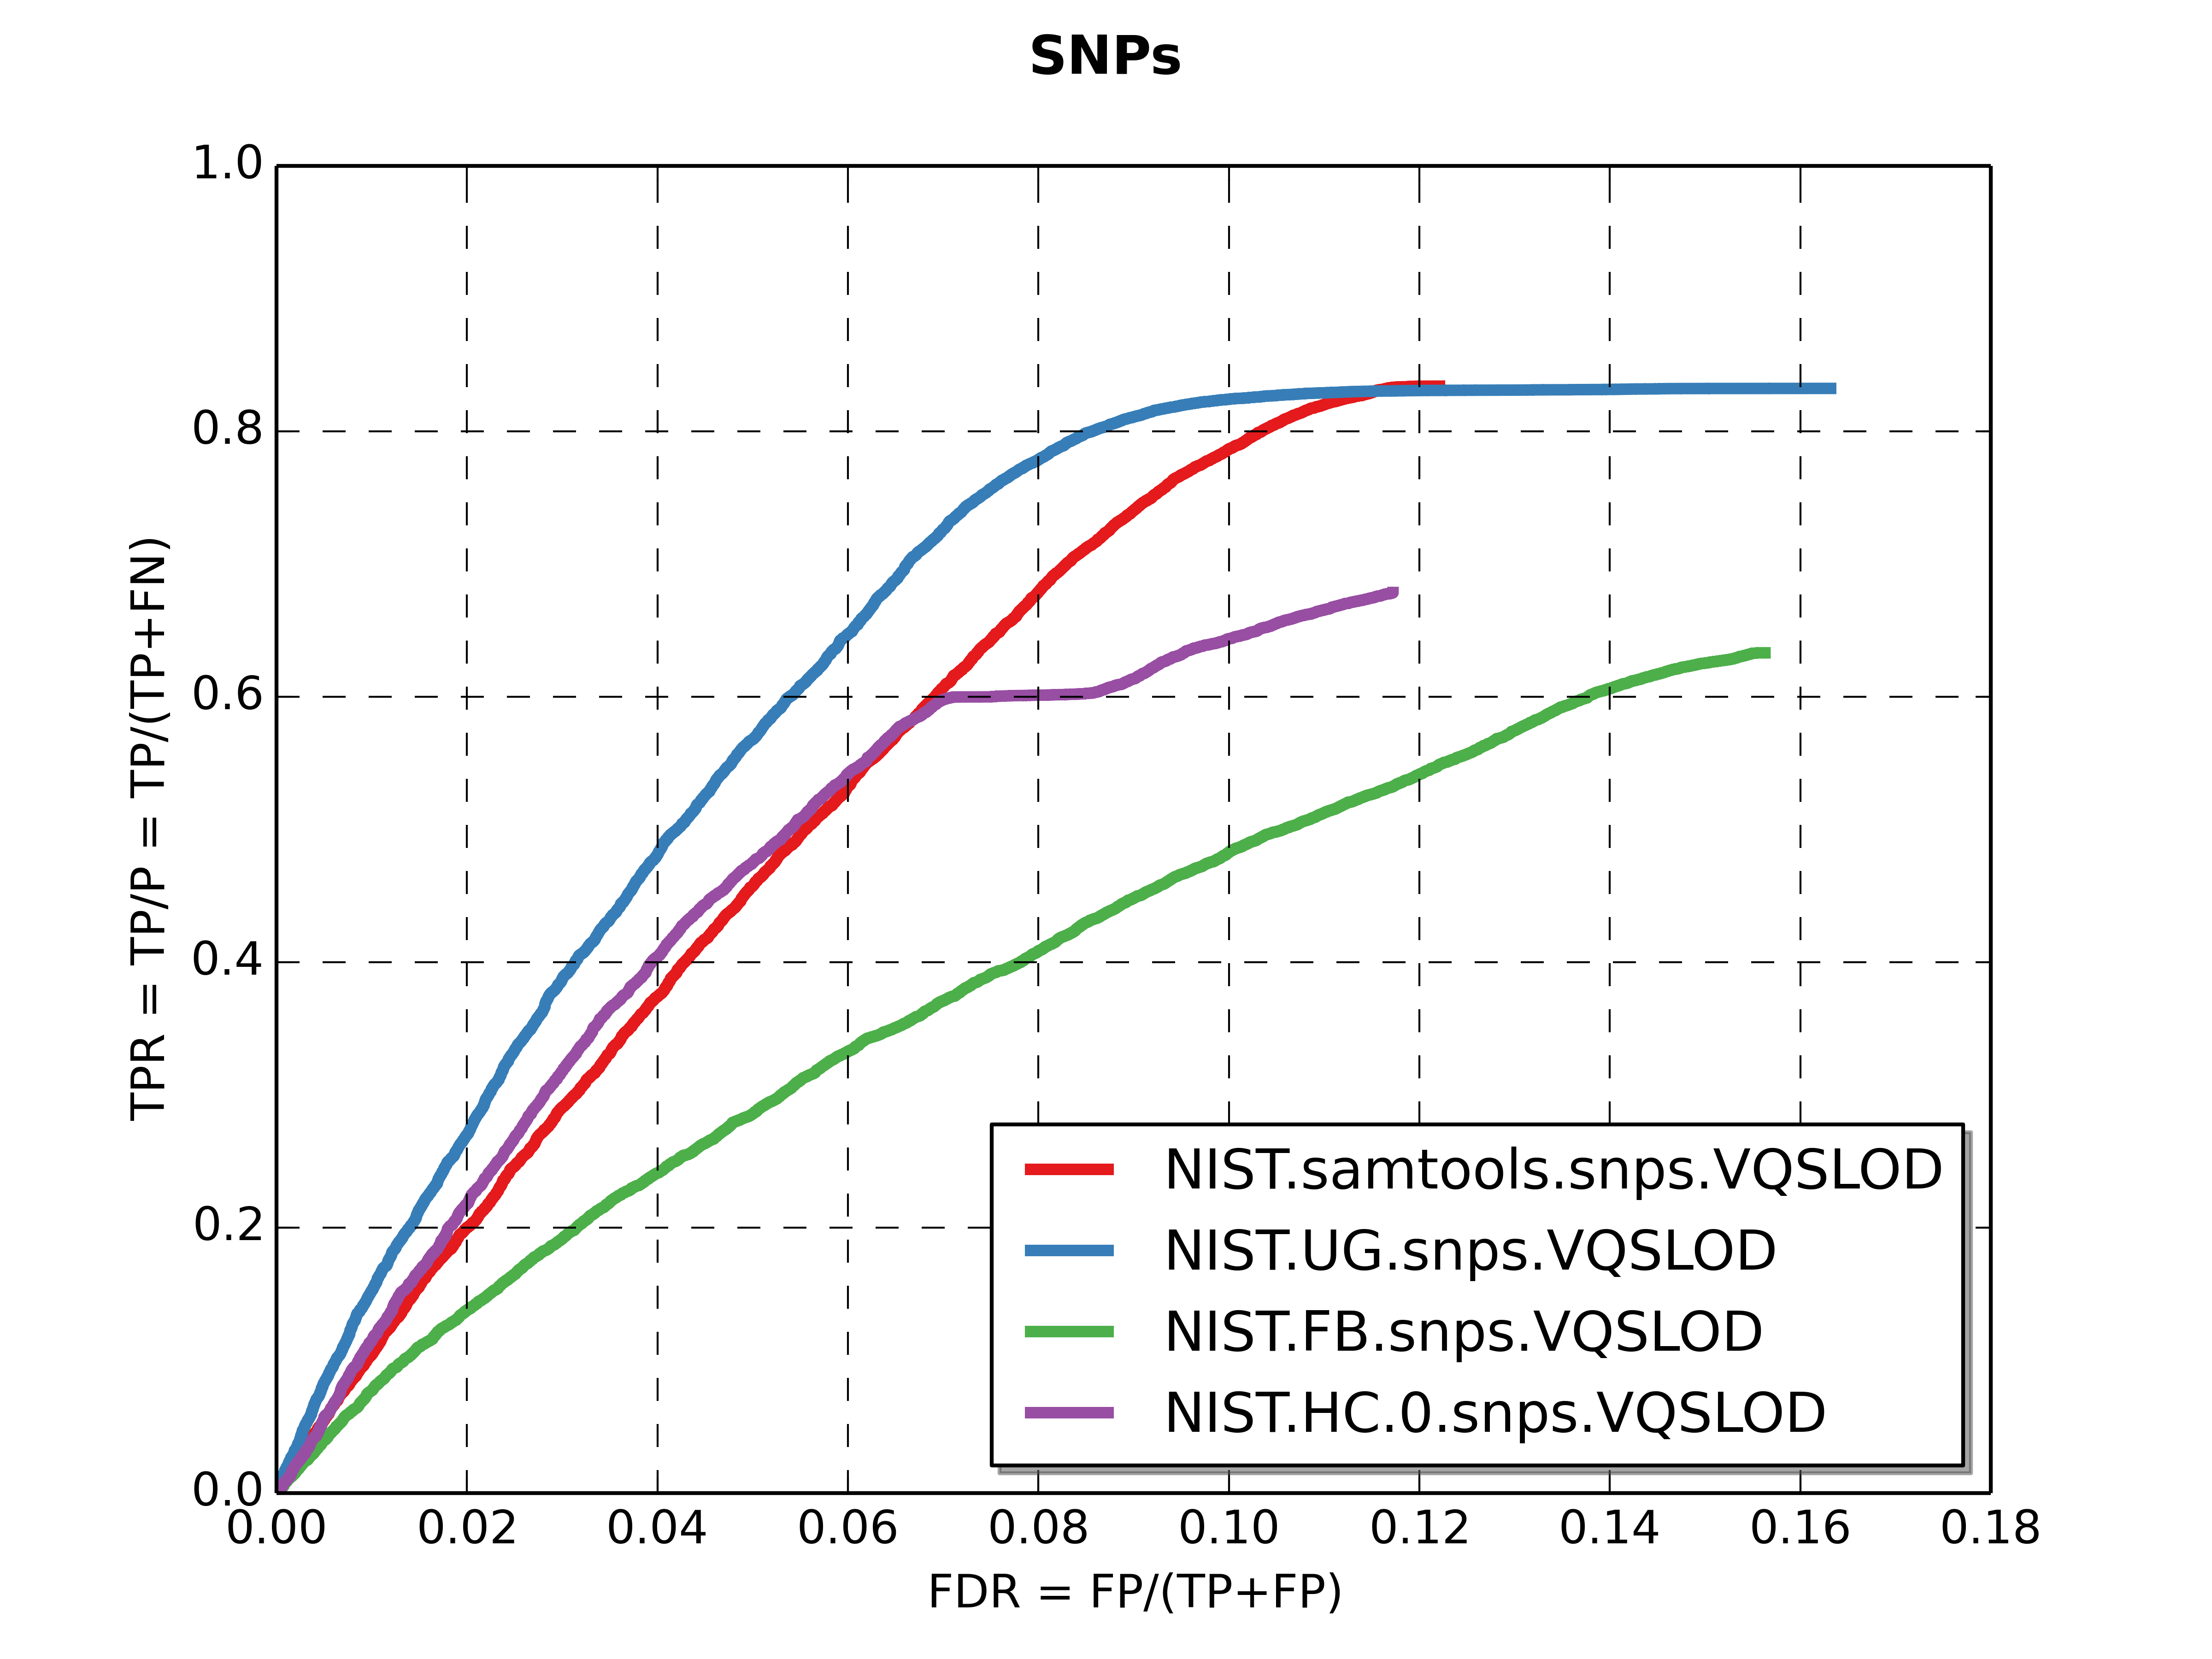
\includegraphics[width=\textwidth]{FDR_snps}
%        \caption{SNPs}
%        \label{fig:roc_snps}
%    \end{subfigure}%
%    \begin{subfigure}[b]{0.45\textwidth}
%        \includegraphics[width=\textwidth]{FDR_indels}
%        \caption{Indels}
%        \label{fig:roc_indels}
%    \end{subfigure}%
\end{figure}

%For high coverage data, we evaluated the NA12878 sample alone re-sequenced on the X-10 pipeline with the highly curated set of variants produced by GiaB.1 We showed that the X-10 and the new pipeline used with it produced high quality data that when normalised showed a high degree of sensitivity versus the GiaB reference set and a low false discovery rate (Table \ref{table:FDRhigh}). When the Illumina 50x Platinum set, sequenced on the Illumina Hiseq 2000 platform was reprocessed through the same pipeline it produced similarly high results, though the INDEL sensitivity and false discovery rate were slightly better. We believe this may be because of the higher coverage and PCR free library preparation used in the creation of this sequence.

%\input{tables/FDRhigh}

\subsubsection{Variant calling}
After deciding on the best algorithm we will carry out variant calling. We will carry out joint variant calling across as many samples as possible to enable a greater sensitivity for low frequency variants and improve the ability to filter out false variants. We have also previously shown that calling across populations and doing genotype refinement yields better concordance and correlation with SNP arrays.

\begin{figure}[!htbp]
\centering
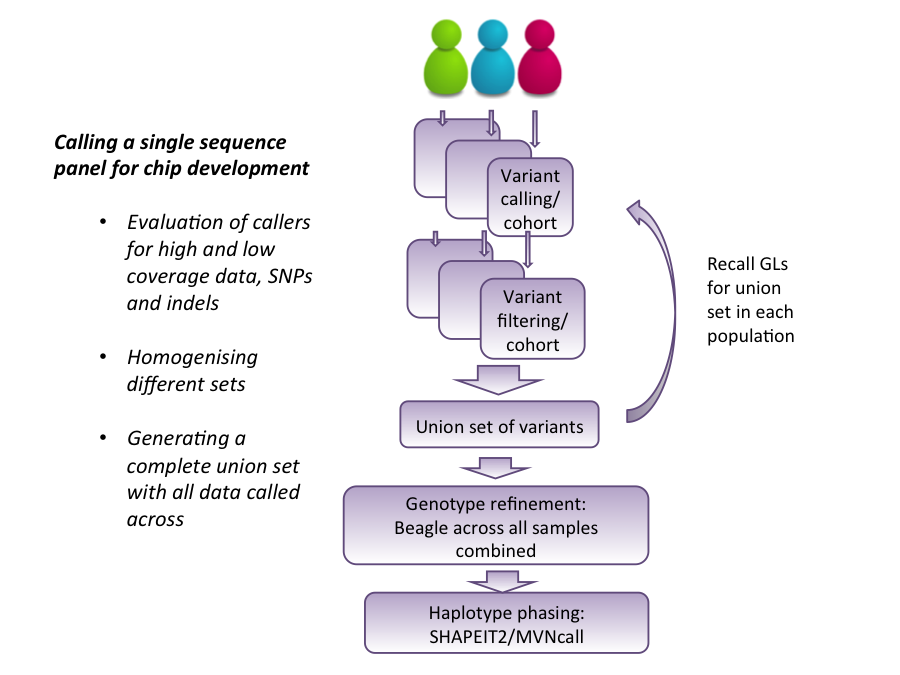
\includegraphics[width=0.8\textwidth]{ADRP/figures/calling}
\caption{Homogenised calling across all datasets to generate a single panel}
\label{fig:calling}
\end{figure}
%Datasets generated with unique Illumina chemistry, and those with different coverages will need to be called in separate subsets.
GATK3.4 \gls{UG} will be used for calling SNPs from the low coverage data, respectively. Multiple samples will be called simultaneously with \gls{UG}. During variant calling \gls{UG} by default downsamples each sample randomly to a maximum coverage of 250 (\-\-downsampling\_type BY\_SAMPLE and \-\-downsample\_to\_coverage 250). We will use the default minimum base quality for UG, which is currently 17 (\-\-min\_base\_quality\_score 17). %10 for HC
At each site we don't call more than the 6 best alternate alleles (\-\-max\_alternate\_alleles 6).
For low coverage data we use calling and emission thresholds (\-stand\_call\_conf and \-stand\_emit\_conf) of 10 as the sample count is greater than 100 as per \href{https://www.broadinstitute.org/gatk/guide/pdfdocs/GATK_GuideBook_2.7-4.pdf}{GATK best practises}. %page 13
%Indels will be called with a plethora of software packages (see the next section).

%If pedigree information is available, then this will be used by UnifiedGenotyper %and GenotypeGVCFs
%in calculation of the InbreedingCoeff annotation, which is used for subsequent variant filtering. Pedigree information will also be used for refinement and phasing. Incomplete pedigrees will be inferred from IBD matrices for sequenced and non-sequenced samples in each cohort.

%\subsubsection{Calling of short indels and structural variants}
With UG we will only make a call in the low coverage data, if the number of consensus indels exceeds a threshold of 5 (--min\_indel\_count\_for\_genotyping 5), which is the default value and the value used for phase 1 of 1000G.
%1000G low coverage indel calling by the Broad - "if a candidate indel allele was present in at least 5 reads at a site, it would be passed over to the next step for genotyping, or otherwise it was excluded."
We furthermore use PINDEL, GINDEL, Dindel, samtools, MATE-CLEVER and SOAPdenovo to call indels shorter than 100bp and deletions longer than 100bp. Breakdancer is used to identify structural variants (SVs) in trios. GenomeSTRiP is used for discovery of deletions. We will use best practices of each method to filter variants prior to creating a consensus set. For Pindel for example it will be a requirement that an indel appear in more than 3 samples and with more than 10 supporting reads in total among all samples.
%GoNL Indels (1-20bp) "GATK UG and at least one other algorithm"
%GoNL Deletions (20-100bp) "more than one method" "at least 3 families and transmitted to at least 1 child"
%GoNL Deletions (>100bp) "at least two algorithms" "at least 3 families and transmitted to at least 1 child"

We remove indels with the maximum number of alternate alleles.
%1000G called indels as biallelic.
Similar to 1000G we will remove protein-coding frameshift indels exclusive to low coverage samples and do post-hoc filtering of short indels with a support vector machine (SVM) or random forest (RF) machine learning approach and by applying a MAF threshold of 0.5\%. The latter machine learning method has been used successfully at the Broad Institute. One could classify indels by:
\begin{enumerate}
\item length (continuous or classified)
\item type (homopolymer run (HR) with runs of 6 or more identical nucleotides, tandem repeat (TR))
\item frameshift/nonframeshift in coding regions
\item tandem repeat length (dinucleotide repeat, trinucleotide repeat, STR/microsatellite (2-5/6/9), minisatellite (10-60)
%INSERTION-DELETION VARIANTS IN 179 HUMAN GENOMES - Table 3 - Characteristics of indels
\item HR insertion (more likely), HR deletion (less likely)
\item tandem repeat type (CG, non-CG)
\item SNP at same site, no SNP at same site
\item biallelic, multialleic
\item inside/outside RepeatMasker regions
\item P site / non-P site; i.e. the reference base not N, depth not less than half of average, depth not twice of average, less than 20\% of reads at position have MQ of 0, base not covered. Calculate averages for the autosomes and the X chromosome independently.
\item allele balance
\item strand bias
\item mapping quality
\item number of supporting non-reference reads
\item distance to nearby indels
\item cytoband: gneg, gpos25, gpos50, gpos75, gpos100, acen, gvar
\end{enumerate}

The NIST NA12878 truth set currently does not hold information on structural variants (SVs). We therefore carry out calling of SVs with multiple callers, apply default calling thresholds and use a consensus dataset as the final SV dataset.

Other variant callers to consider are listed in the table below.
\input{tables/INDELcallers}

Variant calling is carried out jointly across 2,478 individuals; i.e. 1,140 males and 1,338 females.

The SNP count after variant calling is summarised in table \ref{tab:SNPcount}.

\paragraph{Calling of chromosomes X and Y}
The X chromosome will be called jointly for males and females with the same ploidy, because the current version of \gls{UG} is not functional for ploidies different from 2. Likewise the pseudoautosomal regions (PARs) 1 and 2 on the X chromosome will be called like the autosomes; i.e. jointly for males and females with all samples treated as diploid. Variant calling of the Y chromosome will only be carried out for males. The PARs on the Y chromosome are masked in the reference sequence and not subject to calling. An excessive number of heterezogyous calls of haploid genotypes can be utilized for a QC step of sites and samples; thresholds to be decided.
%The mitochondrial variants will be called with GATK, VarScan2\cite{Koboldt2012} and MitoSeek and the union set recalled and annotated with GATK prior to filtering. VarScan is chosen, because it performs well at extreme read depths.\cite{Stead2013} MitoSeek is a software package dedicated to calling variants from mtDNA reads. When calling with GATK the ploidy will be set to the mean coverage in the MT contig divided by the mean coverage in the somatic chromosomes.
%ftp://ftp.1000genomes.ebi.ac.uk/vol1/ftp/technical/reference/phase2_reference_assembly_sequence/README_human_reference_20110707
%http://gatkforums.broadinstitute.org/discussion/1214/can-i-use-gatk-on-non-diploid-organisms
%GoNL - "Consensus sequences were called by GATK."

%\input{tables/ploidies}



\subsubsection{Variant Filtering}

%TODO: For HaplotypeCaller we should check if splitting snps/indels sites into snps and indels yield a greater SNP accuracy rather than salvaging the SNPs from the INDEL-filtered snps/indels sites. Perhaps call SNP and BOTH separately...

Filtering will be carried out with GATK3.4 \gls{VR}. GATK best practices will be used for filtering SNPs.
%http://gatkforums.broadinstitute.org/discussion/1259/which-training-sets-arguments-should-i-use-for-running-vqsr
We will use HapMap III and 1000G phase 1 Omni2.5 sites as truth and training sets (prior probabilities of 15 and 12). High confidence 1000G phase 1 SNPs will be used as an additional training set (prior 10). This dataset does not contain Y chromosome variants. %For indels we will use the Mills and Devine and 1000G gold standard as a truth and training set (prior 12). In both cases
dbSNP138 or newer will act as a set of known sites.
To build our Gaussian mixture model we use annotations at each site related to coverage (QD=QualByDepth and DP), strand bias (FS=FisherStrand, SOR=StrandOddsRatio), mapping quality (MQ, MQRankSum, ReadPosRankSum).
%For indels we use the same annotations, except for MQ being left out.
DP is the approximate read depth after filtering reads with poor mapping quality and bad mates. QD is the variant confidence normalized by the unfiltered depth for the variant allele. FS is a Phred-scaled p-value using Fisher's exact test to detect strand bias. SOR is the odds ratio of a 2x2 contingency table (rows and columns are positive/negative strand and reference/alternate allele) to detect strand bias. MQ is the RMS of the mapping qualities, which serves an an average across reads and samples. MQRankSum is the Z-score from a Wilcoxon rank sum test of alternate vs. reference mapping qualities. ReadPosRankSum is the Z-score from a Wilcoxon rank sum test of alternate vs. reference read position biases.
%When not doing variant calling with HaplotypeCaller we
We will also use the annotation HaplotypeScore, which is a statistical measure of more than 2 haplotypes being present at the same site for a sample.

The NA12878 sample will be included at an appropriate coverage, when doing variant calling. PCR-free reads will be used for the validation sample to avoid PCR artefacts. The inclusion of NA12878 allows for selection of a filtering threshold, which yields a good balance between sensitivity and specificity after filtering. Specifically ROC curves will be generated for sample NA12878, for which highly curated SNPs
%and short INDELs
are available for chromosomes 1-22 and X. The ROC curves will be sorted by the variant quality score log odds ratios calculated by VariantRecalibrator.
%For structural variants we will use PacBio 54x NA12878 WGS data as a truth set. %ftp://ftp.1000genomes.ebi.ac.uk/vol1/ftp/technical/working/20131209_na12878_pacbio/si/

%For cohorts with 10 or more founder samples the InbreedingCoeff annotation will also be used. It is a likelihood-based Hardy-Weinberg test for the inbreeding among samples. It will be tested by generation of additional ROC curves, whether the inclusion of the InbreedingCoeff annotation worsens the ability to do VQSR correctly, when there are many related samples. Whenever available pedigree information will be used during variant calling to assist in the calculation of the InbreedingCoeff annotation.

%We apply the filtering by doing a binary heap merge of unfiltered variants to 1) allow two VQSR processes to run simultaneously; i.e. one for SNPs and one for indels and to 2) avoid lexicographical sorting of already numerically sorted files (i.e. VCF and recal files are sorted numerically by genomic coordinate). Alternatively one can run GATK VariantRecalibrator and ApplyRecalibration in sequence twice, which is twice as slow. Furthermore the heap merge only requires a line from the SNP .recal file, the INDEL .recal file and the VCF file to be held in memory at once.
%The excludemarkers option of the current release of Beagle4 cannot be used to apply the filtering, because 1) UG emits two separate VCF records for SNPs and indels at the same site and 2) the excludemarkers option of Beagle4 only allows one to specify variants by rsID or genomic coordinate. The excludemarkers option would otherwise save disk space and time.

Unlike 1000G phase 1 and GoNL we will not filter out multiallelic variants, because we don't find them to be of lower quality than biallelic SNPs and because there is a greater probability of these appearing across thousands of samples from multiple populations from the African continent than in hundreds of samples from one European country. For example 1 in every \~50 SNP in ~2000 Ugandan samples sequenced to a depth of 4x is multiallelic.
%They probably did this, because Beagle3 didn't support multiallelic variants...

\gls{VR} will be applied separately for the autosomes and the X chromsome, because we have shown \gls{VR} culprits to be different for the autosomes and the X chromosome \ref{fig:VRculprits}, because their depth of coverage and hence their depth derived annotations are different.

\begin{figure}[!htbp]
\centering
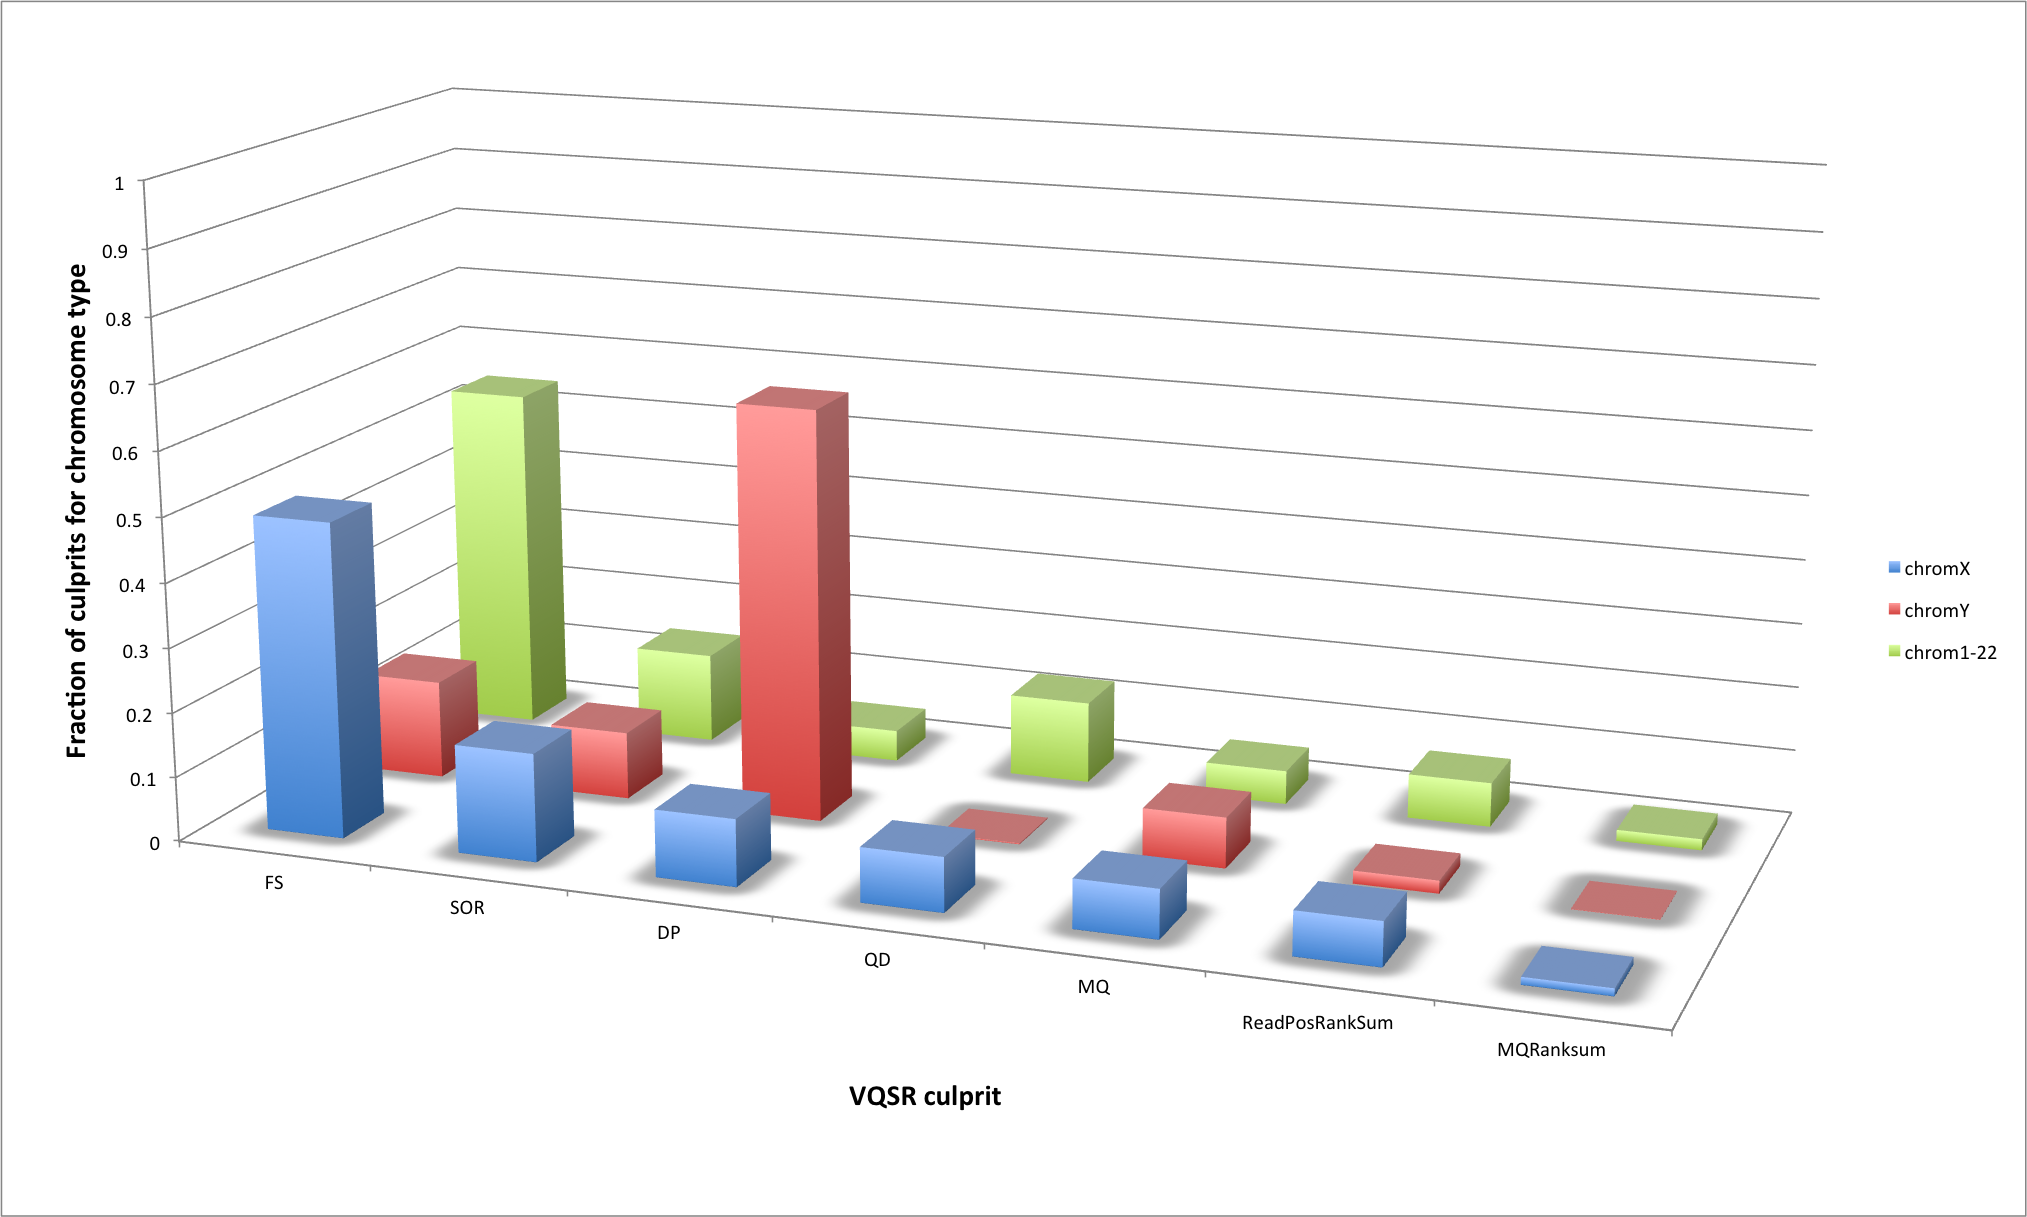
\includegraphics[width=0.8\textwidth]{VRculprits}
\caption{The autosomes and sex chromosomes have different depths of coverage, because only one copy of the non-\gls{PAR} Some of the annotations used by \gls{GATK} \gls{VR} are depth dependent. This figure shows the normalised frequency distribution of culprits as determined by \gls{VR}.}
\label{fig:VRculprits}
\end{figure}

The SNP count after variant filtering is summarised in table \ref{tab:SNPcount}.

\begin{figure}[!htbp]
\centering
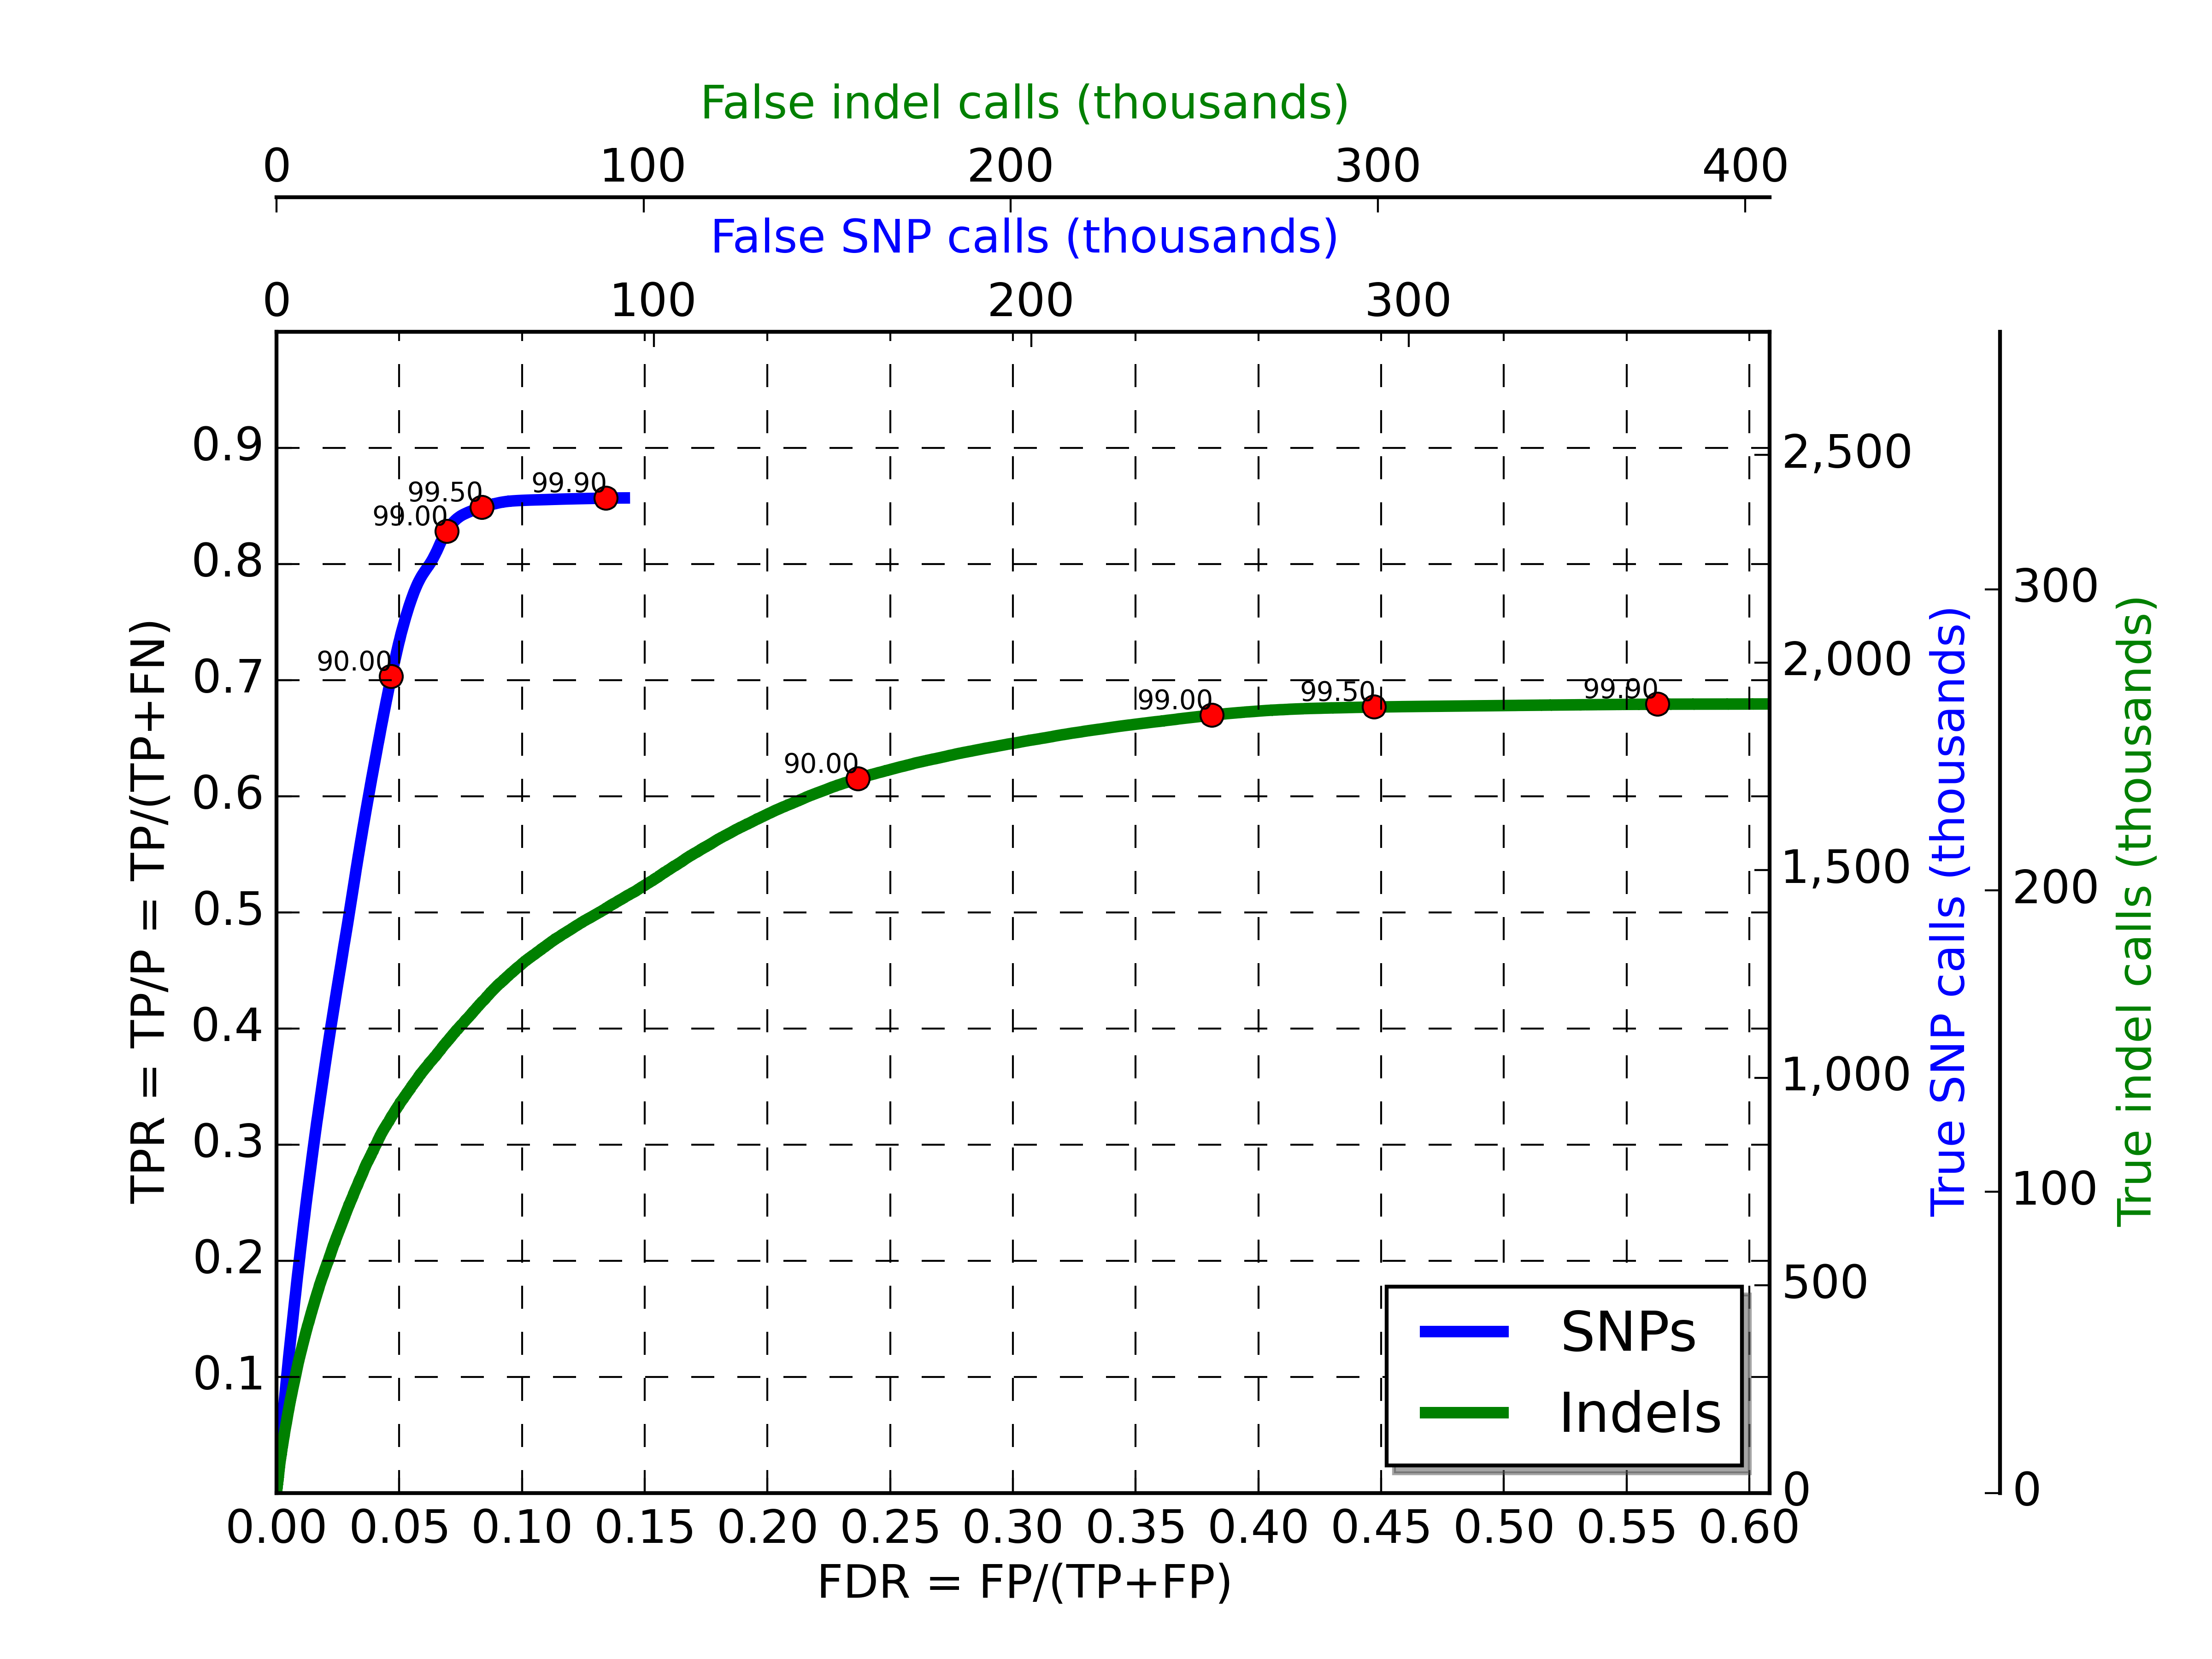
\includegraphics[width=0.8\textwidth]{FDR_ADRP_UG34}
\caption{We used sample NA12878 for which a gold standard truth set is available to calculate sensitivity and specificity as a function of VQSLOD. We use the plot to select the optimal truth sensitivity threshold. This plot is for calls on the ADRP samples using GATK \gls{UG} 3.4}
\label{fig:ROC1}
\end{figure}

\subsubsection{Merging of datasets by recalling prior to refinement and phasing}
Following curation of individual datasets, these will need to be merged to homogenise variant calls across all data, and generate a non-sparse matrix of variant calls, where the union of variants across all samples is available for each population. This process is similar to the merger of reference panels by imputation (Figure \ref{fig:merging_reference_panels}), which could have been used, if raw reads had not been available for all populations. In order to fill the sparse matrix a union set of calls will be generated for variants that have passed filtering in each dataset (Figure \ref{fig:calling}). Prior to merging we recode any haploid male genotypes (non-PAR X and Y) to homozygous diploid genotypes if necessary. %Prior to merging 1) indels will be left aligned (e.g. bcftools norm) and 2) SNPs and indels called in low coverage data by UnifiedGenotyper will be merged into single records with bcftools (bcftools norm -m +any).
%and 3) variants called from reads aligned to build 38 will be lifted over to build 37 (liftOver). %http://hgdownload.soe.ucsc.edu/admin/exe/linux.x86_64/liftOver
Variants will be merged across cohorts (with bcftools merge $|$ bcftools view -G instead of GATK CombineVariants \texttt{--}minimalVCF, because the latter creates multiple records at the same position, but UG in GGA mode only considers the first record).
%WARN  10:17:31,834 GenotypingGivenAllelesUtils - Multiple valid VCF records detected in the alleles input file at site 20:570945, only considering the first record 
These sites will then be recalled in each dataset to generate genotype likelihoods at these sites.
%Sample NA12878 will not be part of the recalling and NA12878 singletons will not be called by exclusion from the union set.
%Where necessary the union set of sites will be lifted over to build 38 prior to recalling and the recalled variants will then be lifted back over to build 37.
\gls{UG} will be used for recalling in GGA mode (\texttt{-{}-}genotyping\_mode GENOTYPE\_GIVEN\_ALLELES and \texttt{--}output\_mode EMIT\_ALL\_SITES).
%http://gatkforums.broadinstitute.org/discussion/4936/not-all-sites-emitted-with-genotype-given-alleles
The maximum number of allowed alternate alleles will be kept at the default 6, since indels are not being called. %Although it should only be necessary for HaplotypeCaller, interval padding will be added to ensure all known sites are called (--interval\_padding 100). %Not necessary for UG.
%http://gatkforums.broadinstitute.org/discussion/comment/18353
Following this, genotype refinement will be carried out, because we have shown refinement to improve genotype likelihoods for especially rare variants for low coverage data\cite{Gurdasani2015}.

\begin{figure}[htbp]
\centering
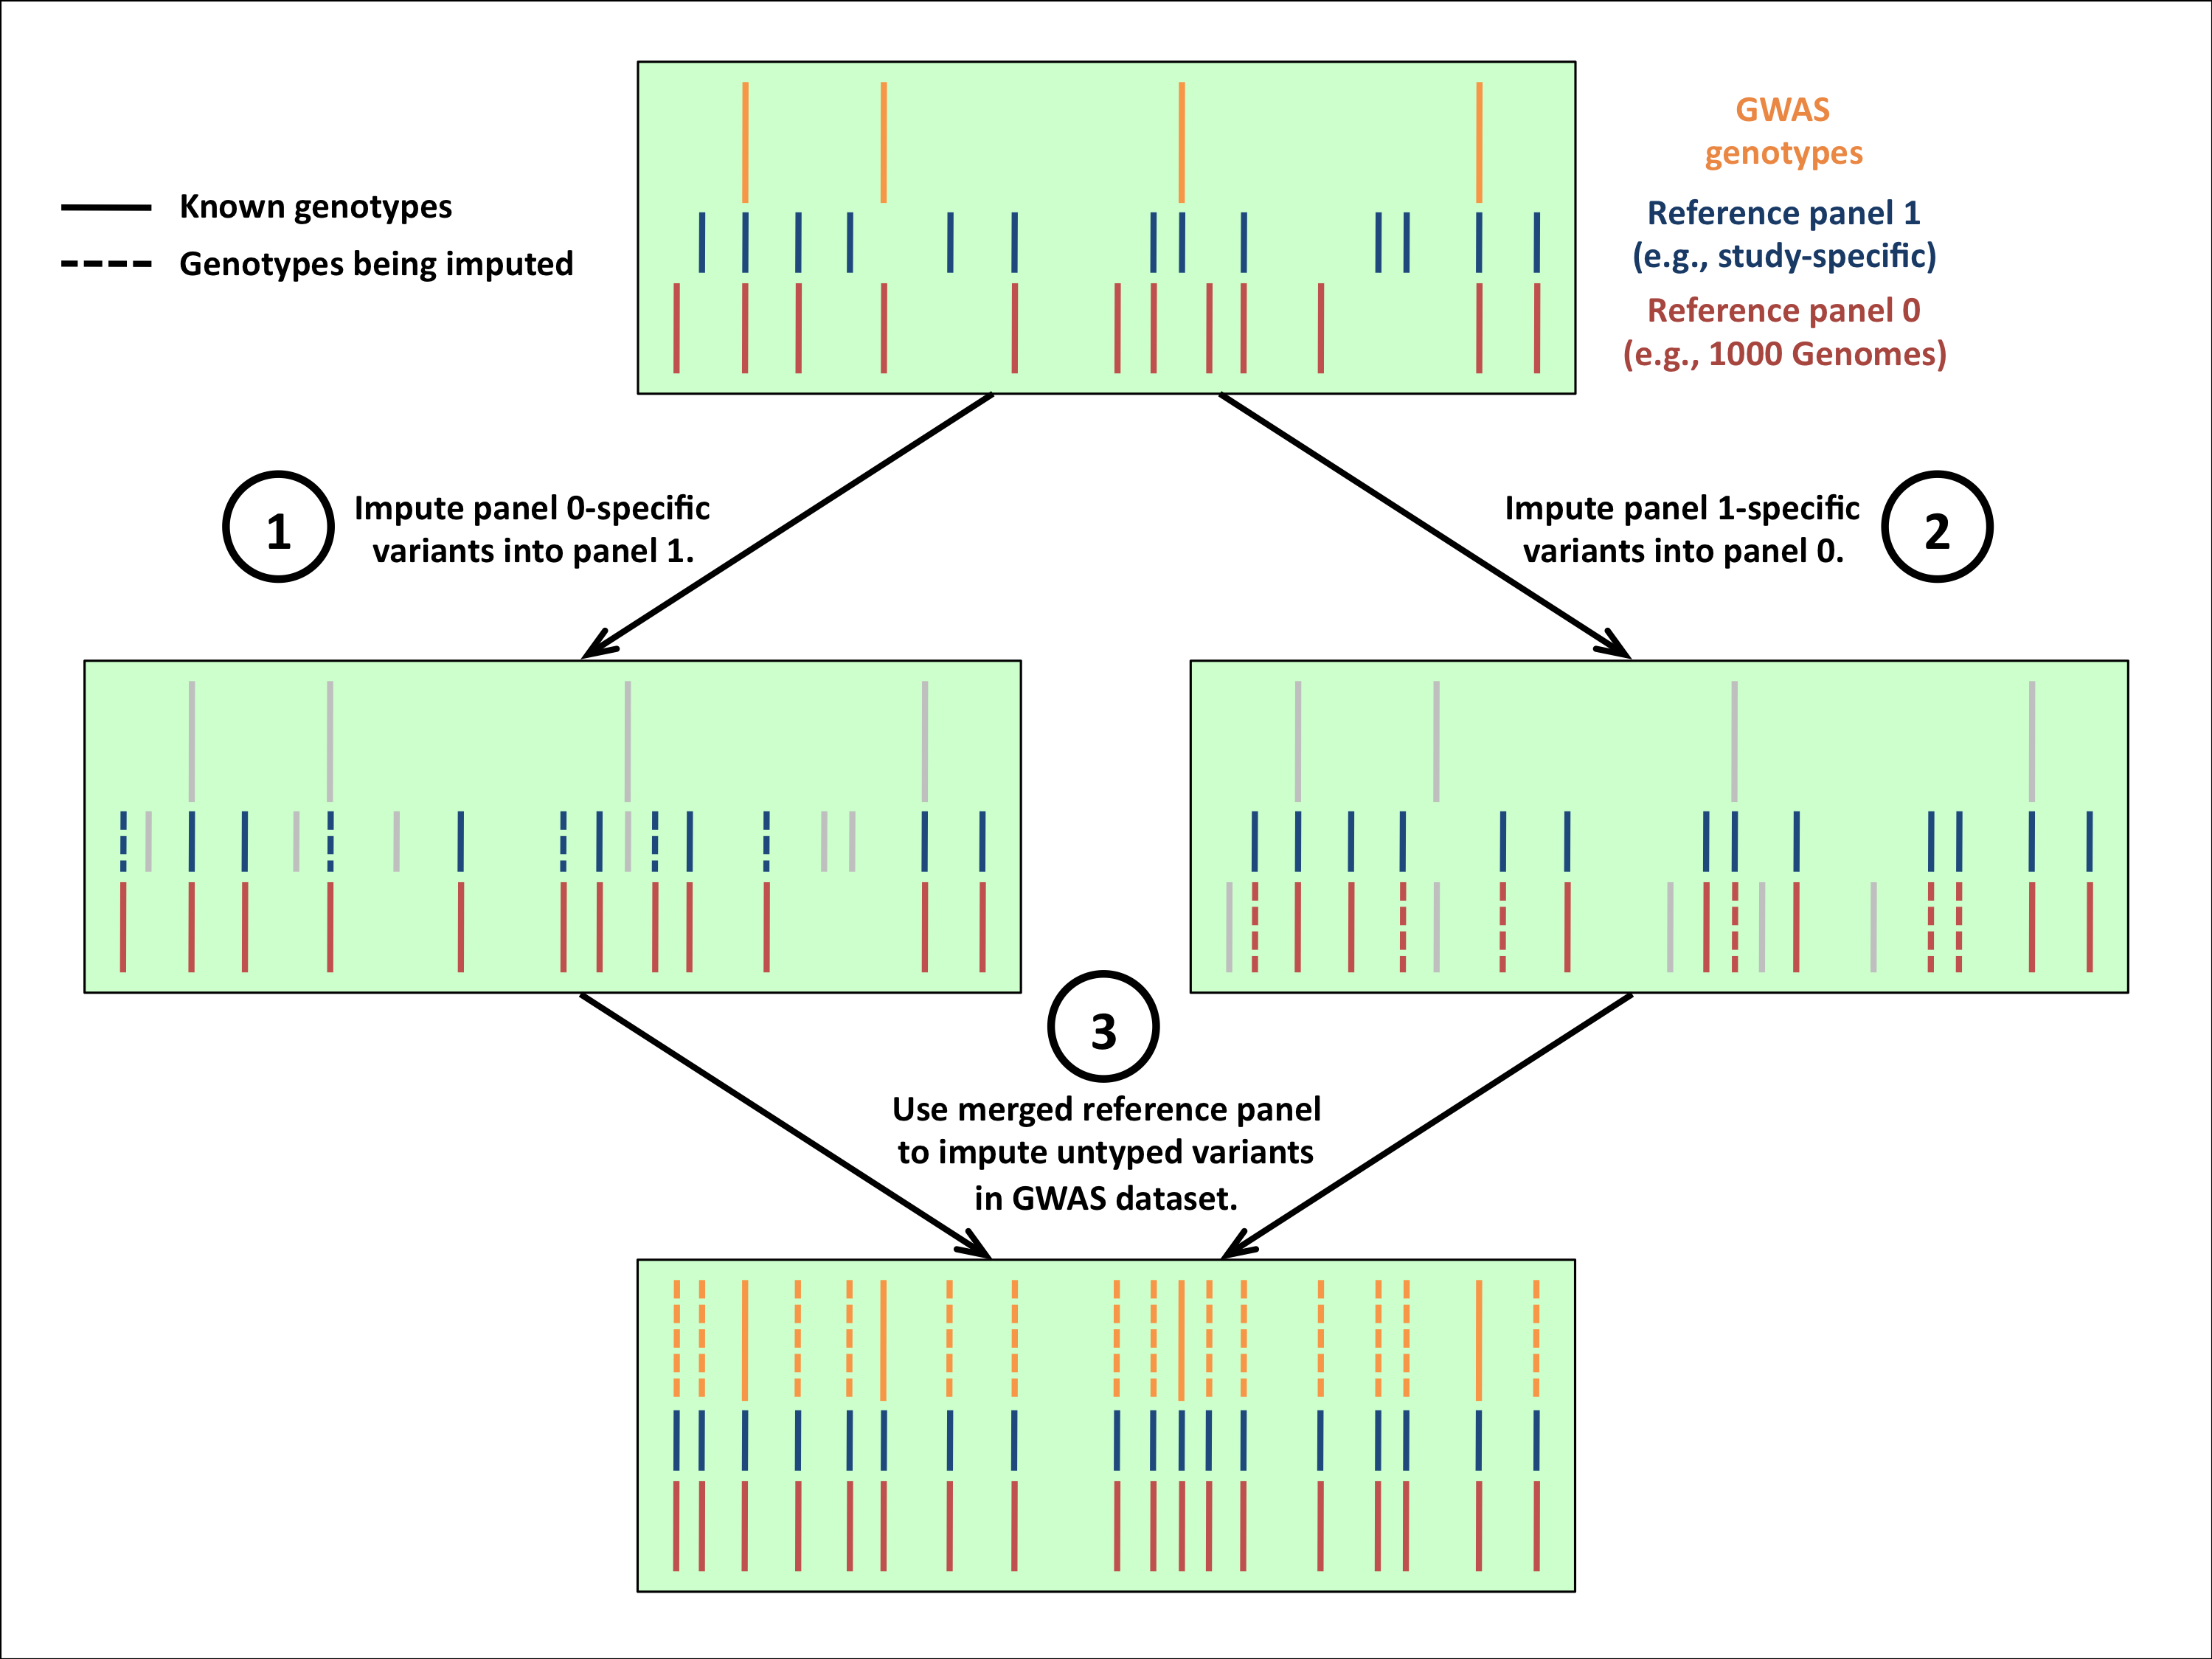
\includegraphics[width=0.6\textwidth]{merging_reference_panels}
\caption[Illustration of the principle of creation of a non-sparse matrix of SNPs across all samples.]{The principle of creating a non-sparse matrix is the same as the merger of reference panels by imputation software. Figure copied from \href{http://mathgen.stats.ox.ac.uk/impute/merging\_reference\_panels.png}{IMPUTE2 web site}.}
\label{fig:merging_reference_panels}
\end{figure}

The detailed work flow is:
\begin{enumerate}
\item{Create \texttt{-{}-}alleles input files for the recalling with \gls{GATK} \gls{UG} run with \texttt{-{}-}genotyping\_mode GENOTYPE\_GIVEN\_ALLELES.}

\begin{enumerate}

\item{Split multiallelic variants into biallelic variants using bcftools norm (-m -) and left align indels (-f) to enable comparison of individual alternate alleles at multiallelic sites by bcftools isec.}

\item{Filter out complex variants from the dataset and 1000Gp3 calls using bcftools view (-v snps).}

\item{Find the union set of sites in the ADRP and 1000Gp3 calls using bcftools isec (-n+1).}

\item{Merge multiallelic sites into one VCF record with bcftools norm (-m +any) to avoid GATK UG only considering the first record.}

\end{enumerate}

\item{Run \gls{GATK} \gls{UG} with \texttt{--}genotyping\_mode GENOTYPE\_GIVEN\_ALLELES across all samples of both datasets.}

%2nd VR because either false sites, false genotypes or UG fail.
\item{Because we found the 1000G samples to cluster together in a PCA plot \ref{fig:PCAprepostVR} we ran another round of \gls{VR} after the joint calling of the union set. We applied a truth sensitivity threshold of 99.5\% after plotting the sensitivity and false discovery rate as a function of VQSLOD scores
%(figure \ref{ROC2}).
. Prior to the second round of \gls{VR} we also exclude variants with a non-reference allele count of 0 (table \ref{tab:SNPcount}), which could be due to a different genotype being called for rare variants during the joint calling of the union set or the variant being called in 1000G by a method involving local realignment, which is not part of \gls{GATK} \gls{UG}. Many of these variants are singletons, which were also excluded as part of the UK10K efforts to generate a merged reference panel.\cite{2015Huang}}

\item{Exclusion of samples in each population with a heterozygosity deviating more than 3.5 standard deviations from the mean for each population (table \ref{tab:samplecount}).}

\item{Refinement with Beagle4 and phasing with SHAPEIT2 as described in section \ref{sec:refine_and_phase}.}

\end{enumerate}

\begin{figure}[h]
\begin{subfigure}{.5\textwidth}
  \centering
  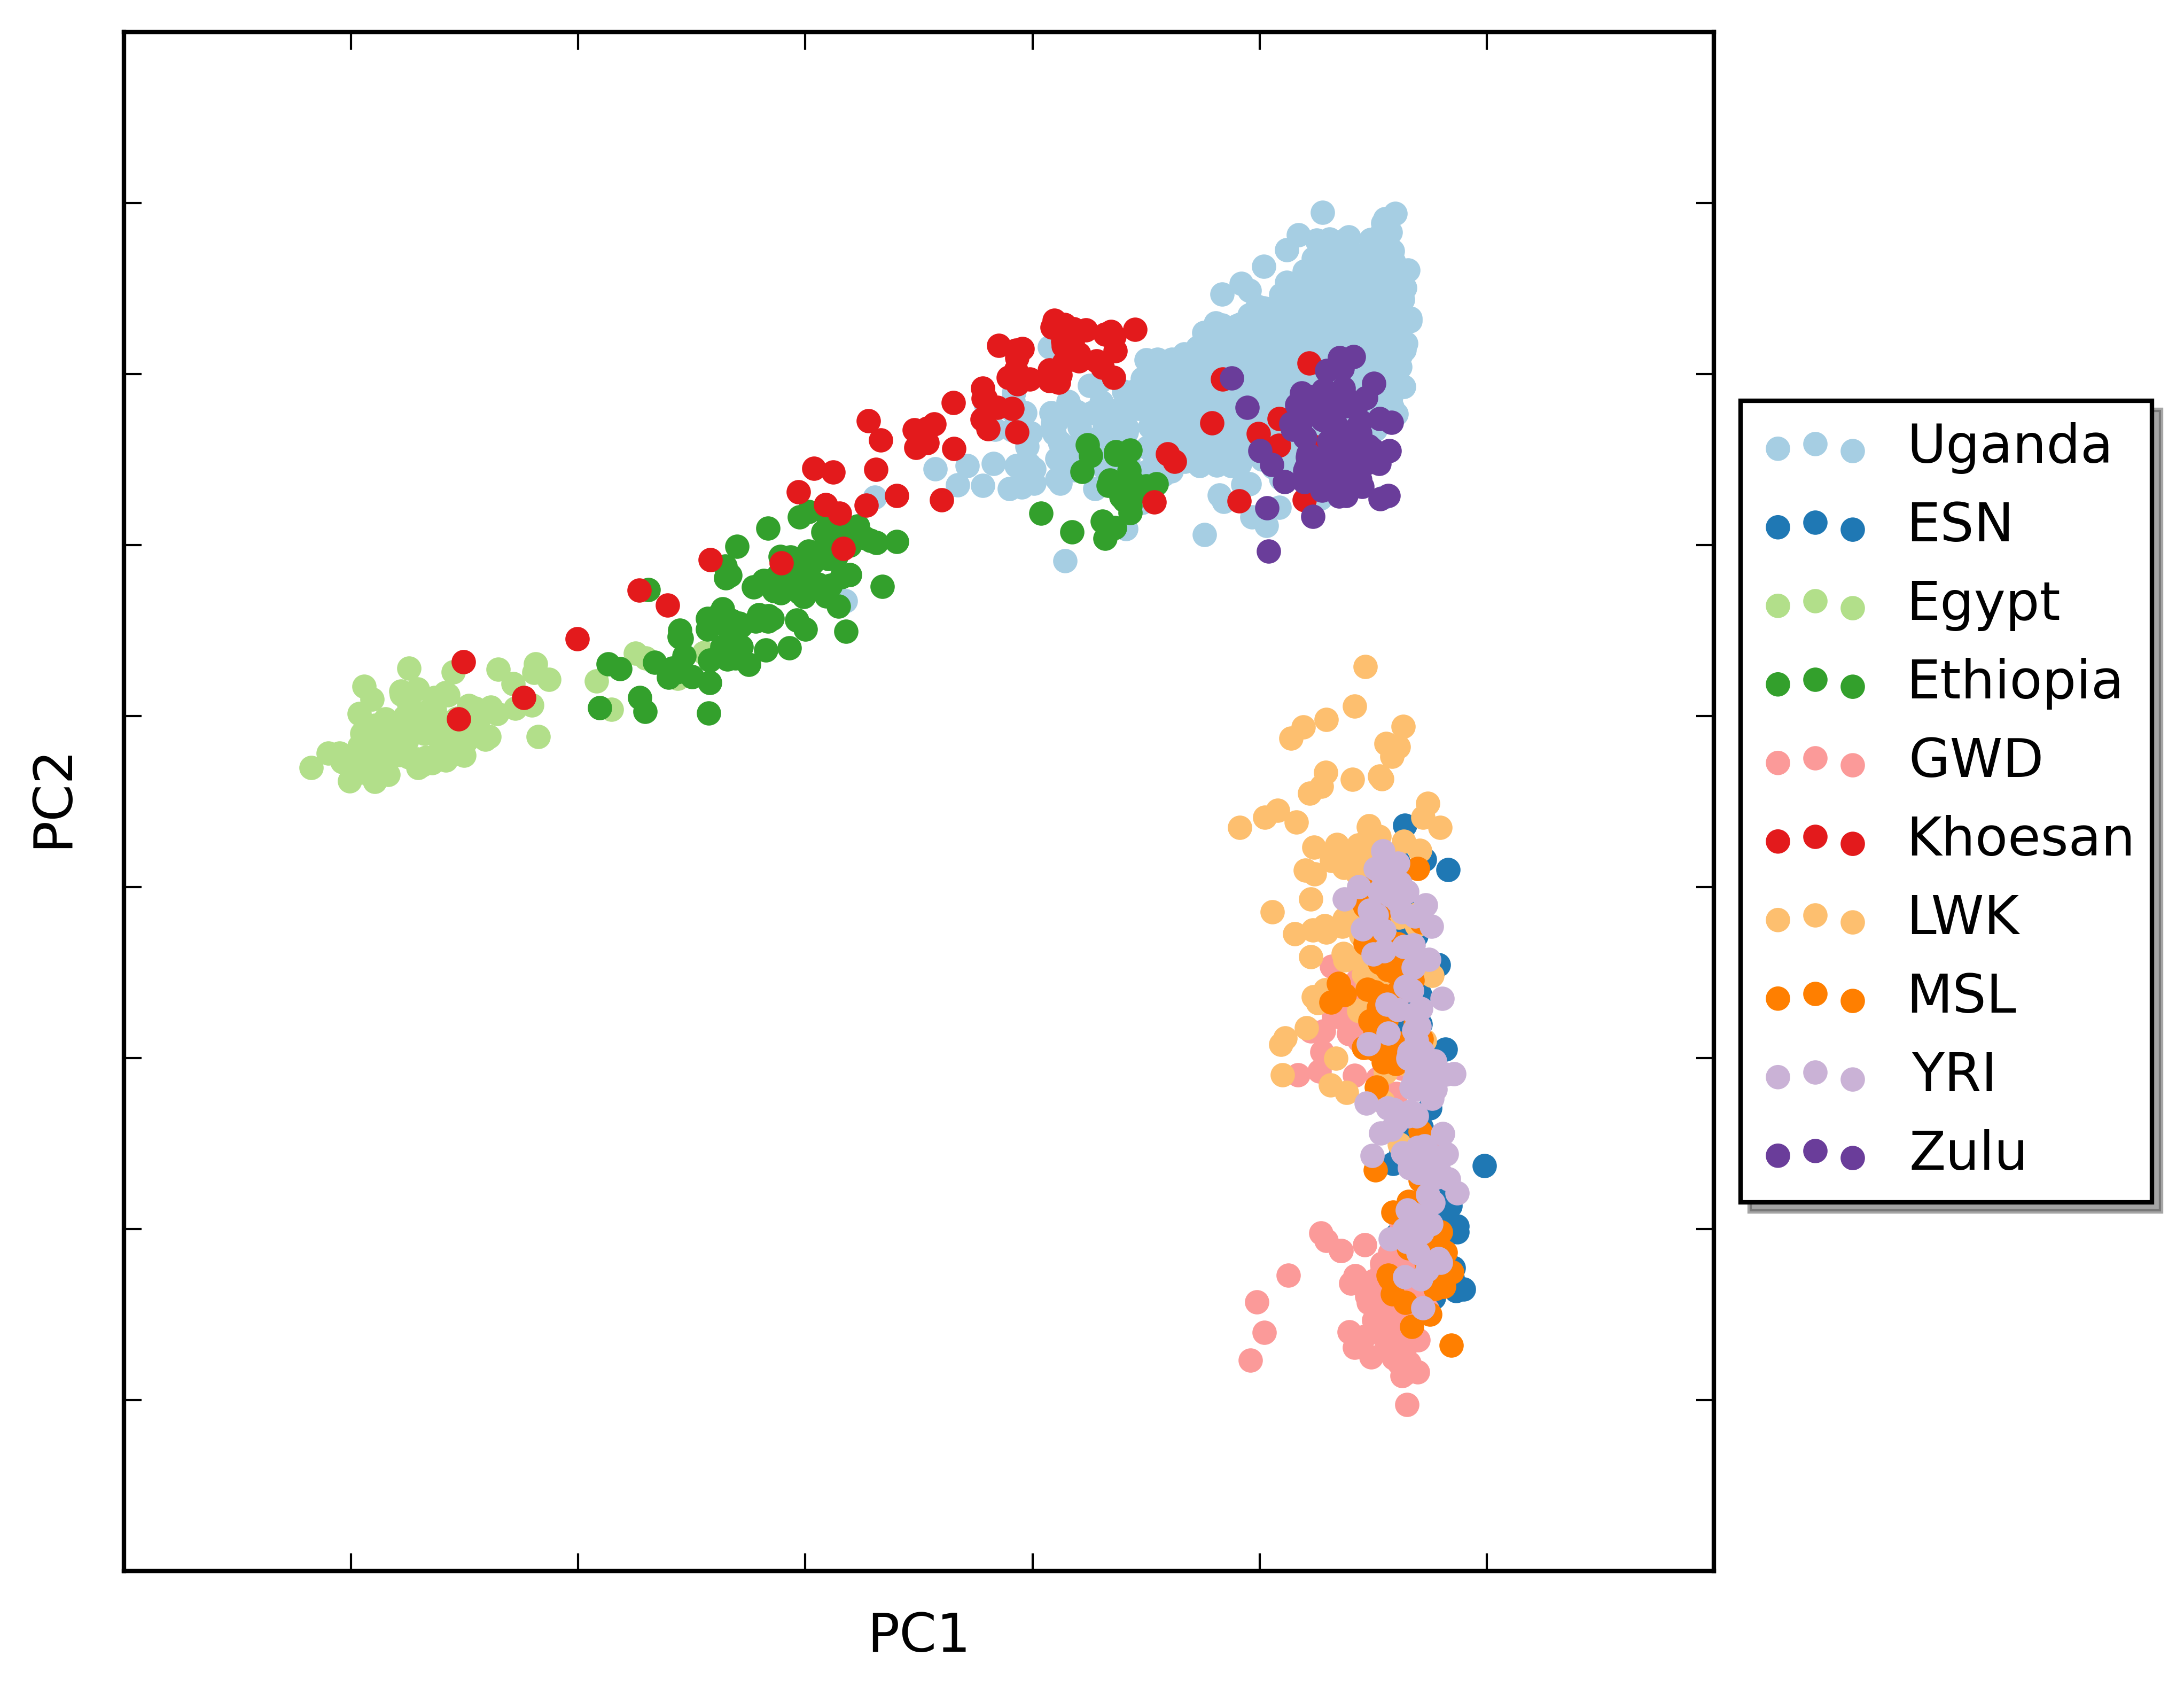
\includegraphics[width=1.0\linewidth]{ADRP/figures/PC12_africa_noVR.png}
  \caption{}
\end{subfigure}%
\begin{subfigure}{.5\textwidth}
  \centering
  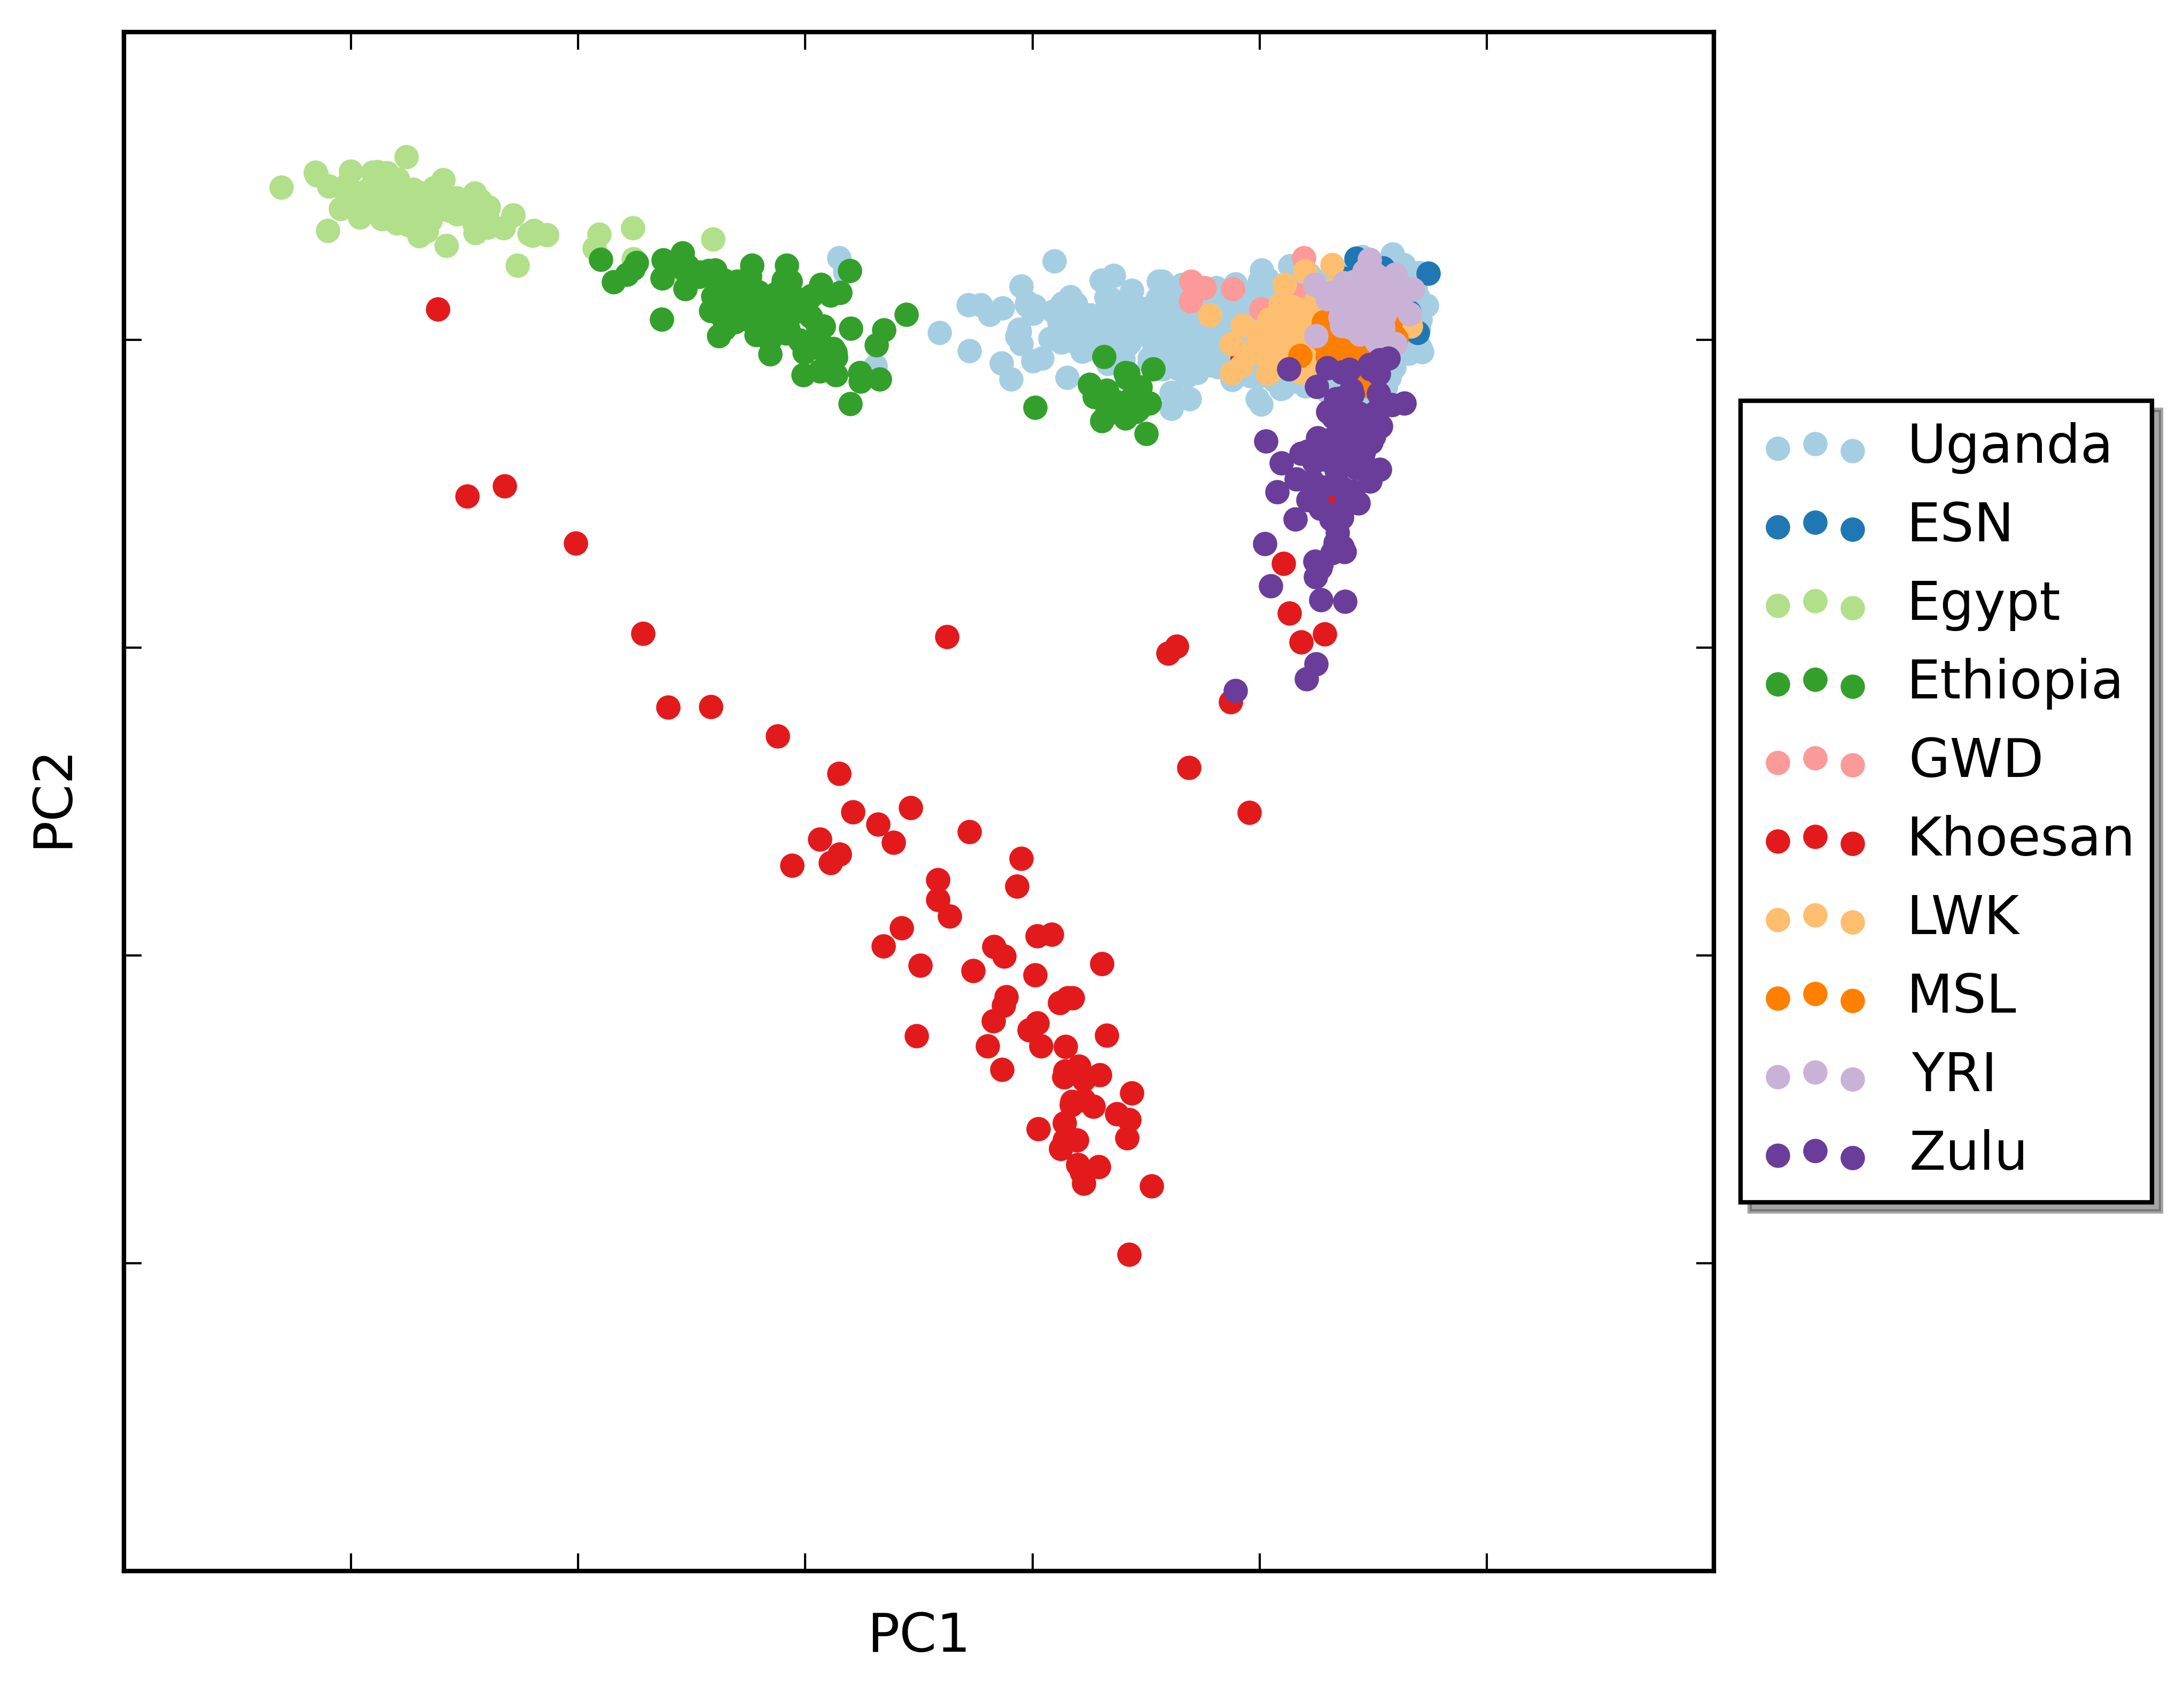
\includegraphics[width=1.0\linewidth]{ADRP/figures/PC12_africa}
  \caption{}
\end{subfigure}%
\caption[\gls{PCA} plot of 10 African populations.]{Plots of principal components 1 and 2 for 3055 African samples prior to refinement without (a) and with (b) a 2nd round of \gls{VR}. The \gls{LWK} samples from East Africa can be seen to cluster with the 4 \gls{1000G} populations from West Africa, if a 2nd round of \gls{VR} is not carried out, which filters out approximately 10 million variants.}
\label{fig:PCAprepostVR}
\end{figure}

The sample count after each step of the curation process is summarised in table \ref{tab:samplecount}.

The SNP count after merger with 1000G and re-calling of the union set of sites jointly across all samples is summarised in table \ref{tab:SNPcount}.

Prior to refinement we check the correlation with chip data (table \ref{tab:correlation_prerefinement} and figure \ref{fig:correlation_prerefinement})

\begin{table}[htbp]
\centering
\begin{tabular}{l|r|r|r|r}
\hline
Population & Sample Intersection Count & Median & Min & Max \\
\hline
Baganda & 435 & 0.806 & 0.544 & 0.946 \\
Zulu & 67 & 0.824 & 0.674 & 0.934 \\
Ethiopia & 61 & 0.922 & 0.760 & 0.957 \\
Khoesan & 79 & 0.885 & 0.544 & 0.965 \\
Egypt & 97 & 0.943 & 0.770 & 0.979 \\
\hline
\end{tabular}
\caption[Correlation between sequence calls and SNP array genotypes prior to refinement.]{Correlation between sequence calls and chip calls for each population on chromosome 20 prior to refinement after exclusion of heterozygosity outliers.}
\label{tab:correlation_prerefinement}
\end{table}

\begin{figure}[h]
    \centering
    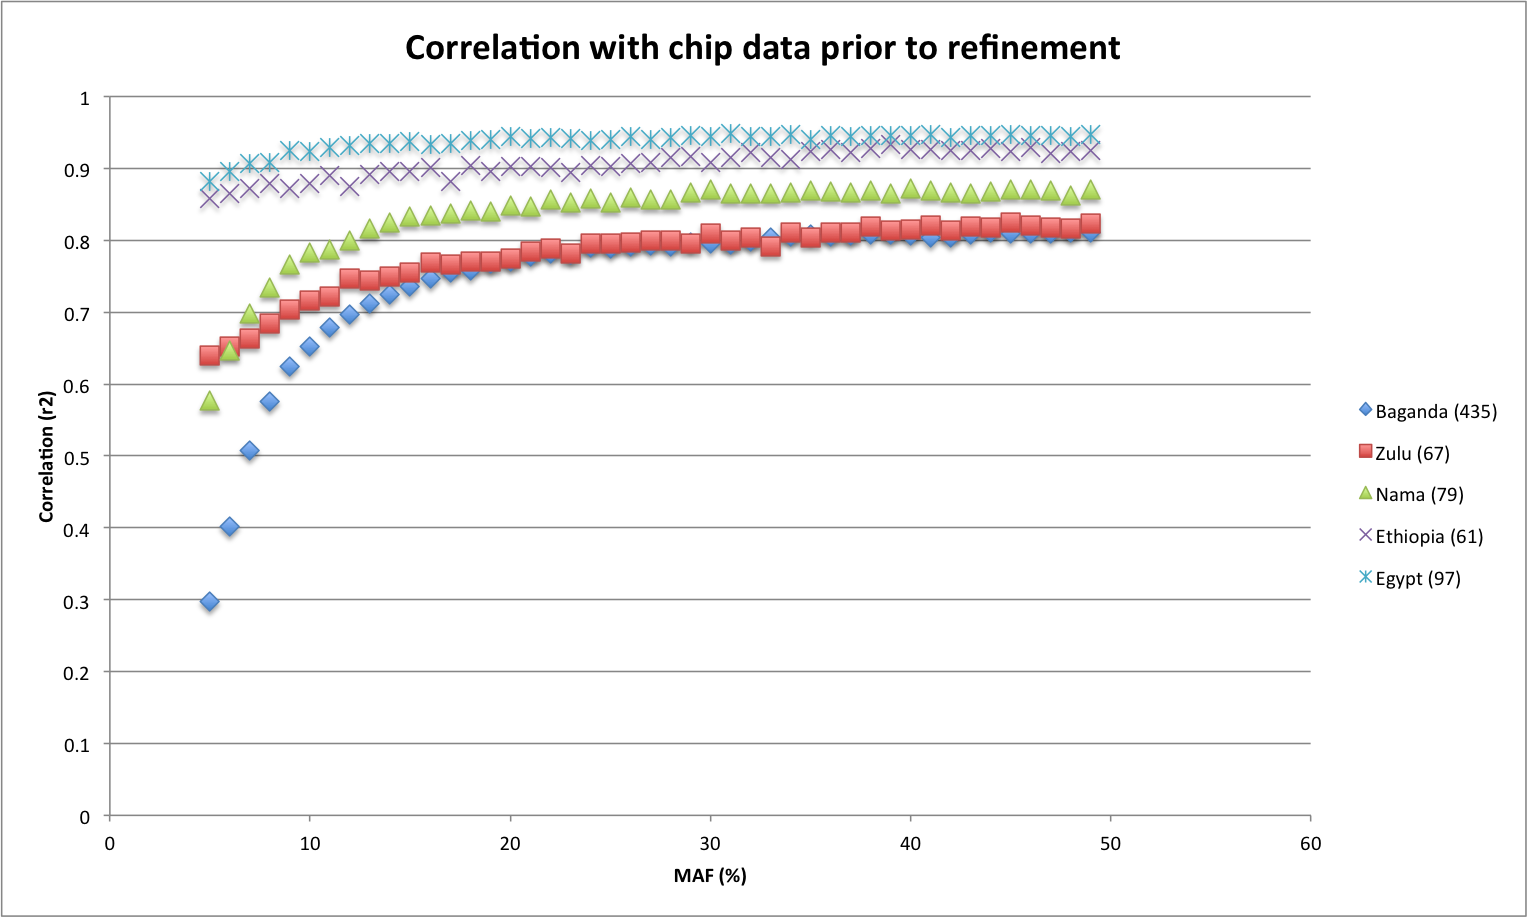
\includegraphics[width=0.8\textwidth]{correlation_prerefinement}
    \caption{Correlation between Omni2.5 chip data and SNP calls prior to refinement as a function of \gls{MAF}.}
    \label{fig:correlation_prerefinement}
\end{figure}

\begin{table}[htbp]
\centering
\begin{tabular}{l|r|r|r|r}
 & Sequencing & QC & verifyBamID & Heterozygosity \\
\hline
Baganda & 1667 & 1656 & 1647 & 1637 \\
Banyarwanda & 199 & 198 & 197 & 196 \\
Barundi & 51 & 51 & 51 & 51 \\
Banyankole & 36 & 36 & 36 & 36 \\
Bakiga & 30 & 30 & 30 & 30 \\
Rwandese Ugandan & 76 & 74 & 74 & 74 \\
Uganda, Other & 41 & 41 & 41 & 41 \\
Zulu & 100 & 98 & 98 & 98 \\
Wolayta & 24 & 24 & 24 & 24 \\
Somali & 24 & 24 & 24 & 24 \\
Oromo & 24 & 24 & 24 & 24 \\
Gumuz & 24 & 23 & 23 & 23 \\
Amhara & 24 & 22 & 22 & 22 \\
Egypt & 100 & 100 & 100 & 100 \\
Khoesan & 111 & 107 & 86 & 85 \\
LWK & 99 & N/A & N/A & 99 \\
GWD & 113 & N/A & N/A & 113 \\
MSL & 85 & N/A & N/A & 85 \\
ESN & 99 & N/A & N/A & 99 \\
YRI & 108 & N/A & N/A & 108 \\
1000Gp3 (nonAFR, ASW, ACB) & 2000 & N/A & N/A & 2000 \\
\hline
 &  &  &  &  \\
Sum & 5035 & 5012 & 4981 & 4969
\end{tabular}
\caption[Count of samples after each step of the curation process.]{Count of samples after each step of the curation process. N/A means that curation step was not carried out for that data set. Sequencing is the number of sequenced samples. QC is the initial QC process adapted from UK10K. verifyBamID is the subsequent check for contaminated samples with excess heterozygosity and swapped samples. Heterozygosity is the check of heterozygosity outliers after recalling variants prior to refinement with Beagle4.}
\label{tab:samplecount}
\end{table}

\begin{table}[htbp]
\centering
\resizebox{\textwidth}{!}{%
\begin{tabular}{l|r|r|r|r|r|r|r}
\hline
Chromosome & UG1 & VR1 & 1000G & Union & UG2 & non-monomorphic & VR2 \\
\hline
1 & 7331048 & 4466570 & 6238533 & 8135665 & 8135665 & 8121685 & 7220178 \\
2 & 7563940 & 4897414 & 6834236 & 8930898 & 8930898 & 8916004 & 8057100 \\
3 & 6126618 & 4062320 & 5624615 & 7347008 & 7347008 & 7335431 & 6679331 \\
4 & 5935191 & 3981077 & 5521818 & 7161759 & 7161759 & 7149973 & 6461409 \\
5 & 5556780 & 3690538 & 5075395 & 6650082 & 6650082 & 6639451 & 6028368 \\
6 & 5373212 & 3516545 & 4835905 & 6282890 & 6282890 & 6272096 & 5660253 \\
7 & 5309419 & 3316764 & 4550705 & 5945705 & 5945705 & 5935472 & 5260940 \\
8 & 4813382 & 3232251 & 4453379 & 5821226 & 5821226 & 5812359 & 5290591 \\
9 & 3974961 & 2468538 & 3441213 & 4495196 & 4495196 & 4487714 & 3979574 \\
10 & 4434086 & 2804022 & 3852282 & 5018268 & 5018268 & 5009565 & 4493579 \\
11 & 4287471 & 2802106 & 3907160 & 5084045 & 5084045 & 5075931 & 4571193 \\
12 & 4347647 & 2710326 & 3724286 & 4863404 & 4863404 & 4854889 & 4363342 \\
13 & 2979117 & 2006917 & 2747376 & 3578012 & 3578012 & 3571947 & 3268732 \\
14 & 2933699 & 1855954 & 2558184 & 3334587 & 3334587 & 3328925 & 2994394 \\
15 & 2784077 & 1680149 & 2337651 & 3049792 & 3049792 & 3044491 & 2693114 \\
16 & 3169848 & 1856110 & 2619149 & 3422074 & 3422074 & 3416016 & 2976742 \\
17 & 3000276 & 1631664 & 2243354 & 2945166 & 2945166 & 2939413 & 2540165 \\
18 & 2390213 & 1595328 & 2187123 & 2848151 & 2848151 & 2843612 & 2587971 \\
19 & 2636969 & 1319309 & 1765908 & 2328868 & 2328868 & 2323718 & 1936939 \\
20 & 2091941 & 1288813 & 1751797 & 2294718 & 2294718 & 2290949 & 2076370 \\
21 & 1307809 & 770704 & 1063228 & 1376114 & 1376114 & 1373478 & 1205255 \\
22 & 1427343 & 782316 & 1064502 & 1396629 & 1396629 & 1393869 & 1192106 \\
X & 3838312 & 2280287 & 3261471 & 4260245 &  &  &  \\
 &  &  &  &  &  &  &  \\
\hline
Sum & 93,613,359 & 59,016,022 & 81,659,270 & 106,570,502 & 102,310,257 & 102,136,988 & 91,537,646 \\
\end{tabular}
}
\caption[\gls{SNP} count after each \gls{ADRP} data curation step.]{Count of SNPs after each step of the curation process. UG1 is an abbreviation for UnifiedGenotyper calls from the ADRP populations. VR1 is an abbreviation for variants passing the first VariantRecalibrator filtering. 1000G is a count of variants in 1000G. Union is a count of variants in the union set, which are recalled with UG. non-monomorphic is a count of the non-monomorphic SNPs after re-calling. VR2 is an abbreviation for passing the second round of VariantRecalibrator filtering.}
\label{tab:SNPcount}
\end{table}

\subsubsection{Generation of the reference panel by genotype refinement and phasing}
\label{sec:refine_and_phase}
We carry out genotype refinement and phasing with SHAPEIT2\cite{Delaneau2012} and MVNcall.\cite{Menelaou2013} We use the SHAPEIT2 for phasing of biallelic sites and MVNcall for phasing of multiallelic sites. We use SHAPEIT2, because it improves on the accuracy of phasing\cite{2014Delaneau} and ultimately downstream accuracy when used for imputation\cite{2015Huang}. Initial refinement of genotype likelihoods is carried out with Beagle4.\cite{Browning20071084} The posterior probabilities calculated by Beagle4 are then used as input for SHAPEIT2 and MVNcall along with a haplotype scaffold generated from SNP array data available for the same populations (figure \ref{fig:haplotype_scaffold}). The SNP array data undergoes QC per population and is phased with SHAPEIT2 across all populations to generate the haplotype scaffold.

\begin{figure}[!htbp]
\centering
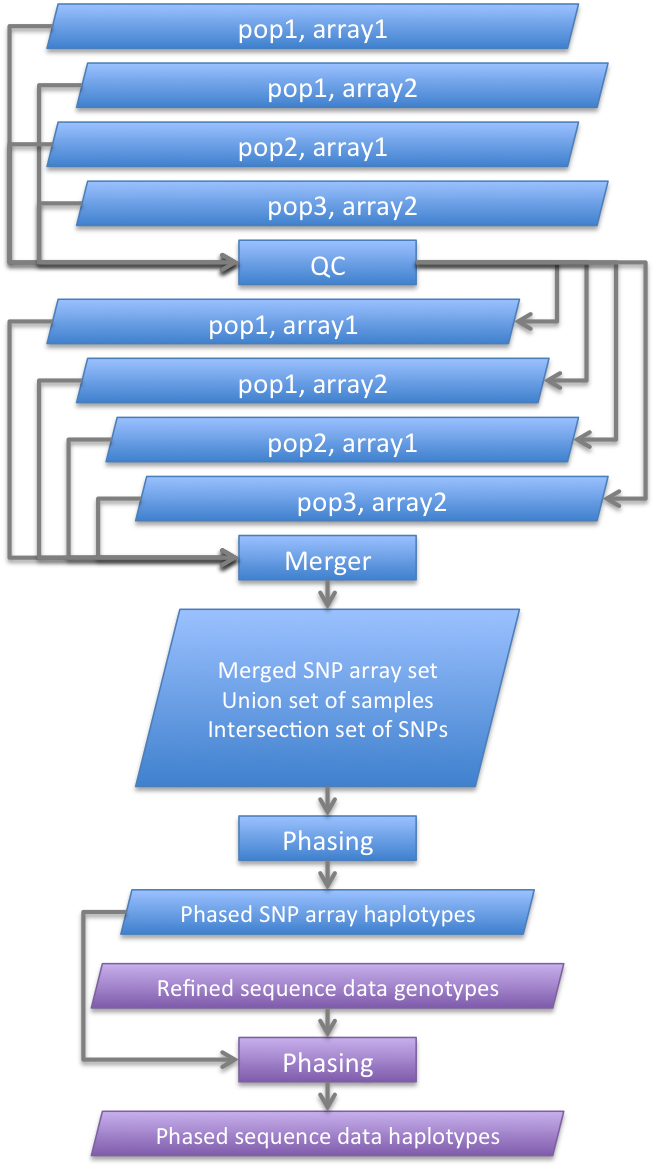
\includegraphics[width=0.4\textwidth]{haplotype_scaffold}
\caption{A haplotype scaffold is used for phasing of the sequence data. The haplotype scaffold is generated from highly accurate SNP array data available for sequenced samples and additional relevant samples and populations (summarized in table \ref{tab:samples_chip} on page \pageref{tab:samples_chip}).}
\label{fig:haplotype_scaffold}
\end{figure}

%MVNcall can also utilize a haplotype scaffold and unlike SHAPEIT2 works for multiallelic sites.\cite{Menelaou2013} However, we use SHAPEIT2, because it improves on the accuracy of phasing.\cite{2014Delaneau}
The Illumina Omni2.5M SNP array has been shown to be an optimal/sufficient haplotype scaffold size in African populations.\cite{Menelaou2013}\cite{2014Delaneau} Pedigree information will be used by SHAPEIT2 when available. For Beagle4 this is less important, as this is only an initial refinement used as input for SHAPEIT2 and MVNcall. We use the duoHMM method of SHAPEIT2 for phasing, because it has been shown to have a lower switch error rate, when pedigree information is available.\cite{OConnell2014} Following generation of this haplotype scaffold, SHAPEIT2 phases the sequence data by filling in missing data in between the scaffold, resulting in more accurate phasing of sequence data.

The chip data will undergo calling and quality control as previously\cite{Gurdasani2015} and as described in section \ref{sec:QCchip}. For the haplotype scaffold, in addition to in-house genotype data available, we will also use called chip data from the 1000G populations YRI (Yoruba in Ibadan, Nigeria) and LWK (Luhya in Webuye, Kenya), which are the only African populations alongside MKK (Maasai in Kinyawa, Kenya), which were genotyped on the Illumina Omni2.5M chip as part of 1000G.
%ftp://ftp.1000genomes.ebi.ac.uk/vol1/ftp/release/20130502/supporting/hd_genotype_chip/

We use the latest release (1274) of Beagle4. We use a sliding window size of 50000 variants and an overlap of 3000 variants between sliding windows. We use the default parameters; e.g. singlescale=0.8, duoscale=1.0, trioscale=1.0, burnin-its=5, phase-its=5, impute-its=5. We sample 4 haplotypes for each individual during each iteration of the algorithm (nsamples=4) and use 1200 variants to build the haplotype frequency model at each locus (buildwindow=1200). After refinement we check that there is a high concordance and correlation between SNP array genotypes and the refined sequence genotype posterior probabilities.

%Figure 8: Overall percent genotype discordance for different scaffold SNP density. Results are presented by population groups: African, European and Asian.
%Is MVNCall only better, if BEAGLE doesn't have phasing information?
%2014Delaneau - "It has been observed that the Beagle method does not have this property, and that Thunder and Impute2 benefit from using an initial set of haplotypes estimated via Beagle."
%2014Delaneu - "This approach generalizes our MVNcall, approach which is designed to phase one variant site at a time onto a haplotype scaffold, and improves upon its accuracy, by phasing multiple sites jointly onto the scaffold and using a more sophisticated underlying model."

%% https://mathgen.stats.ox.ac.uk/genetics_software/shapeit/shapeit.html#gcall

\subsubsection{Quality control after variant calling and genotype refinement}
After merging the datasets by recalling them, we carry out refinement with Beagle4 prior to phasing. We carry out a final QC prior to phasing. If SNP array data is available, we further check after genotype refinement with Beagle4 that the concordance and correlation between chip and sequence genotypes is greater than 0.98 and 0.95 respectively for each sample. We also check for heterozygosity outliers (\textgreater3SD per population) and PCA outliers after genotype refinement. Variant calling and genotype refinement is repeated if a sample either fails the check of genotype concordance, which is a sign of poor data quality, or fails the check of heterozygosity, which can be a sign of sample contamination or a population outlier.

\subsection{Quality control of SNP array data}
%TODO: generate .miss and .multiple from Illumina files and flip according to reference sequence.
The SNP array data to be used for the haplotype scaffold has to undergo quality control. In this section we describe this QC procedure.